\chapter{Results}
\label{chap:results}

\section{Introduction}

The principal aim of this analysis is to measure Higgs boson simplified template cross sections, 
at both stage 0 and stage 1, and their associated uncertainties.
This is achieved by performing a simultaneous fit of the signal and background models 
to the observed \mgg distribution in each category.
A binned maximum likelihood fit is performed in the range $100 < \mgg < \SI{180}{GeV}$, 
with a bin size of \SI{250}{MeV};
this is sufficiently small relative to the diphoton mass resolution 
that a negligible amount of information is lost. %and is computationally much faster

The likelihood function in each category, $\Like_c$, is expressed as:
\begin{equation}
\Like_c(\Largs) = \prod^{N_b}_{i=1} \textrm{Poisson}\left( d_i\,|\, 
                  s_i(\vec{\sigma},\mH,\vec{\theta}) + b_i(\vec{\theta}) \right) \times C(\vec{\theta}),
\end{equation}
where $\vec{\sigma}$ is the set of parameters of interest (POIs), 
which in this analysis are always a set of one or more cross section parameters;
$\vec{\theta}$ is the set of nuisance parameters which affect the measurements 
but are not themselves of interest;
$N_b$ is the number of bins used in the category's \mgg distribution;
Poisson indicates a Poisson function evaluated with the observed number of events 
in the $i^{\mathit{th}}$ bin $d_i$ 
and expected number of events given by the sum of the signal expectation $s_i$ 
and the background expectation $b_i$;
$C(\vec{\theta})$ is the constraint term which penalises deviations 
from the expected values of the signal nuisance parameters,
and applies a penalisation term according to 
the total number of degrees of freedom in the background model.
The expected number of signal events in each bin depends on the POIs, \mH, 
and the nuisance parameters, 
whilst the expected number of background events depends only on unconstrained nuisance parameters.

The total likelihood \Like is then given by the product of the likelihoods over all categories:
\begin{equation}
\Like(\Largs) = \prod^{N_c}_{c=1} \Like_c(\Largs),
\end{equation}
where $N_c$ is the total number of analysis categories.
The fit is then performed by minimising the value of the negative log-likelihood, \NLL, where
\begin{equation}
\NLL = -2\ln\Like(\Largs).
\end{equation}
The free parameters in the fit are the parameters of interest, \
mH, and the background nuisance parameters;
the signal nuisance parameters can vary but are constrained by the $C(\theta)$ term.
The \NLL is constructed and minimised numerically within the RooFit~\cite{RooFit} 
software package for statistical data analysis.
The values of the parameters at the minimum 2NLL are then described as the ``best-fit" values.

A frequentist approach is followed in order to extract the uncertainties on the POIs, 
in addition to their best-fit values.
The likelihood ratio test statistic, \dNLL, is constructed for a range of POI values:
\begin{equation}
\dNLL = -2\ln\frac{ \Like(\textrm{data}\,|\,\vec{\sigma},\hat{\hat{m}}_H,\vec{\hat{\hat{\theta}}}) }
                  { \Like(\textrm{data}\,|\,\vec{\hat{\sigma}},\hat{m}_H,\vec{\hat{\theta}}) },
\end{equation}
where $\hat{\hat{m}}_H$ and $\vec{\hat{\hat{\theta}}}$ are the best-fit values 
of the Higgs boson mass and nuisance parameters at the POI values $\vec{\hat{\sigma}}$;
$\vec{\hat{\sigma}}$, $\hat{m}_H$, and $\vec{\hat{\theta}}$ are the global best-fit values 
of the POIs, Higgs boson mass, and nuisance parameters respectively.
The distribution of the likelihood ratio test statistic 
can then be used to infer the approximate uncertainties on the measurements.
For a sufficient number of events, %in each bin??
the distribution tends to that of a $\chi^2$~\cite{Asymptotic}, 
where the number of degrees of freedom is equal to the number of POIs being measured.
In this case, the 68\% confidence level (CL) intervals 
are given approximately by the corresponding region for a $\chi^2$ distribution, 
which depends on the number of degrees of freedom.
For a single POI, the region is defined by $\dNLL < 1$.
The interpretation of the 68\% CL intervals within the frequentist paradigm 
is that in an ensemble of identical pseudo-experiments, 
the observed interval should should contain the true value of the POI in 68\% of cases.
The crossing points of the \dNLL at $\pm 1$ are therefore quoted
as the 68\% CL uncertainties on the POI in question.

In this analysis the POIs considered are Higgs boson simplified template cross sections, 
which are defined at various levels of granularity and denoted by the symbol $\sigma$.
The so-called ``stage 0" cross sections are equivalent 
to the sum of the individual stage 1 cross sections.
This makes clear that parameters can be defined as sums of different STXS bins, 
not just individual bins themselves.
Measuring a wider set of STXS bins provides more information, 
but the uncertainties are correspondingly larger than if fewer parameters are measured.
Therefore in this section results are reported under various scenarios, 
with between one and thirteen POIs in total.

In each case, the fit is performed with the cross section as the parameter of interest.
After the value of the cross section has been measured, the value is normalised to the SM prediction. 
This procedure differs from that used to measure a signal strength $\mu$, 
as defined in Chapter~\ref{chap:theory},
where the parameter in the fit is the ratio of the observed cross section to the SM prediction.
The key difference between the two is that in the signal strength measurements,
the uncertainty on the SM prediction must be considered in the fit
because it enters directly in the denominator of the parameter of interest.
In contrast, the STXS measurements do not include these uncertainties on the SM yield;
the measured cross sections do not directly depend on the SM prediction.
This ensures the measurements are as independent as possible of the current SM predictions
and their uncertainties, 
which means they remain useful if the theoretical advances are made in the future.

In the following section, the observed diphoton mass distribution
and the composition of the analysis categories are presented.
The remainder of chapter describes the results of stage 0 and stage 1 measurements 
within the STXS framework.
All results were first reported in Ref.~\cite{HIG-18-029}.

\section{Observed diphoton mass distributions}

The observed diphoton mass distribution is displayed together with the result 
of a signal plus background fit in Figure~\ref{fig:results_MassPlot}.
The fit contains one inclusive signal parameter, 
which includes all signal events where $|y_H| < 2.5$.
The fit is performed simultaneously to all analysis categories, 
each of which is summed with a weight 
corresponding to the ratio of signal events to background events. %this shows the "true" sensitvity?
The uncertainty on the background prediction is also shown.
The signal peak due to Higgs boson production is clearly visible.
%The background-only hypothesis is excluded with a significance of more than five standard deviations.

The result of the same single parameter fit is also shown in Figure~\ref{fig:results_MassPlots}.
In this case, only certain subsets of categories are included in the sum.
The \mgg distributions for the weighted sum of the categories targeting 
ggH 0J, ggH 1J, ggH 2J, and VBF production are shown.
The plots indicate the total number of events and approximate signal to background ratio
for the different processes targeted in this analysis.

%The full set of unweighted diphoton mass distributions for each category 
%considered in the analysis are contained in Appendix~\ref{app:massplots}.

\begin{figure}[hptb]
  \centering
  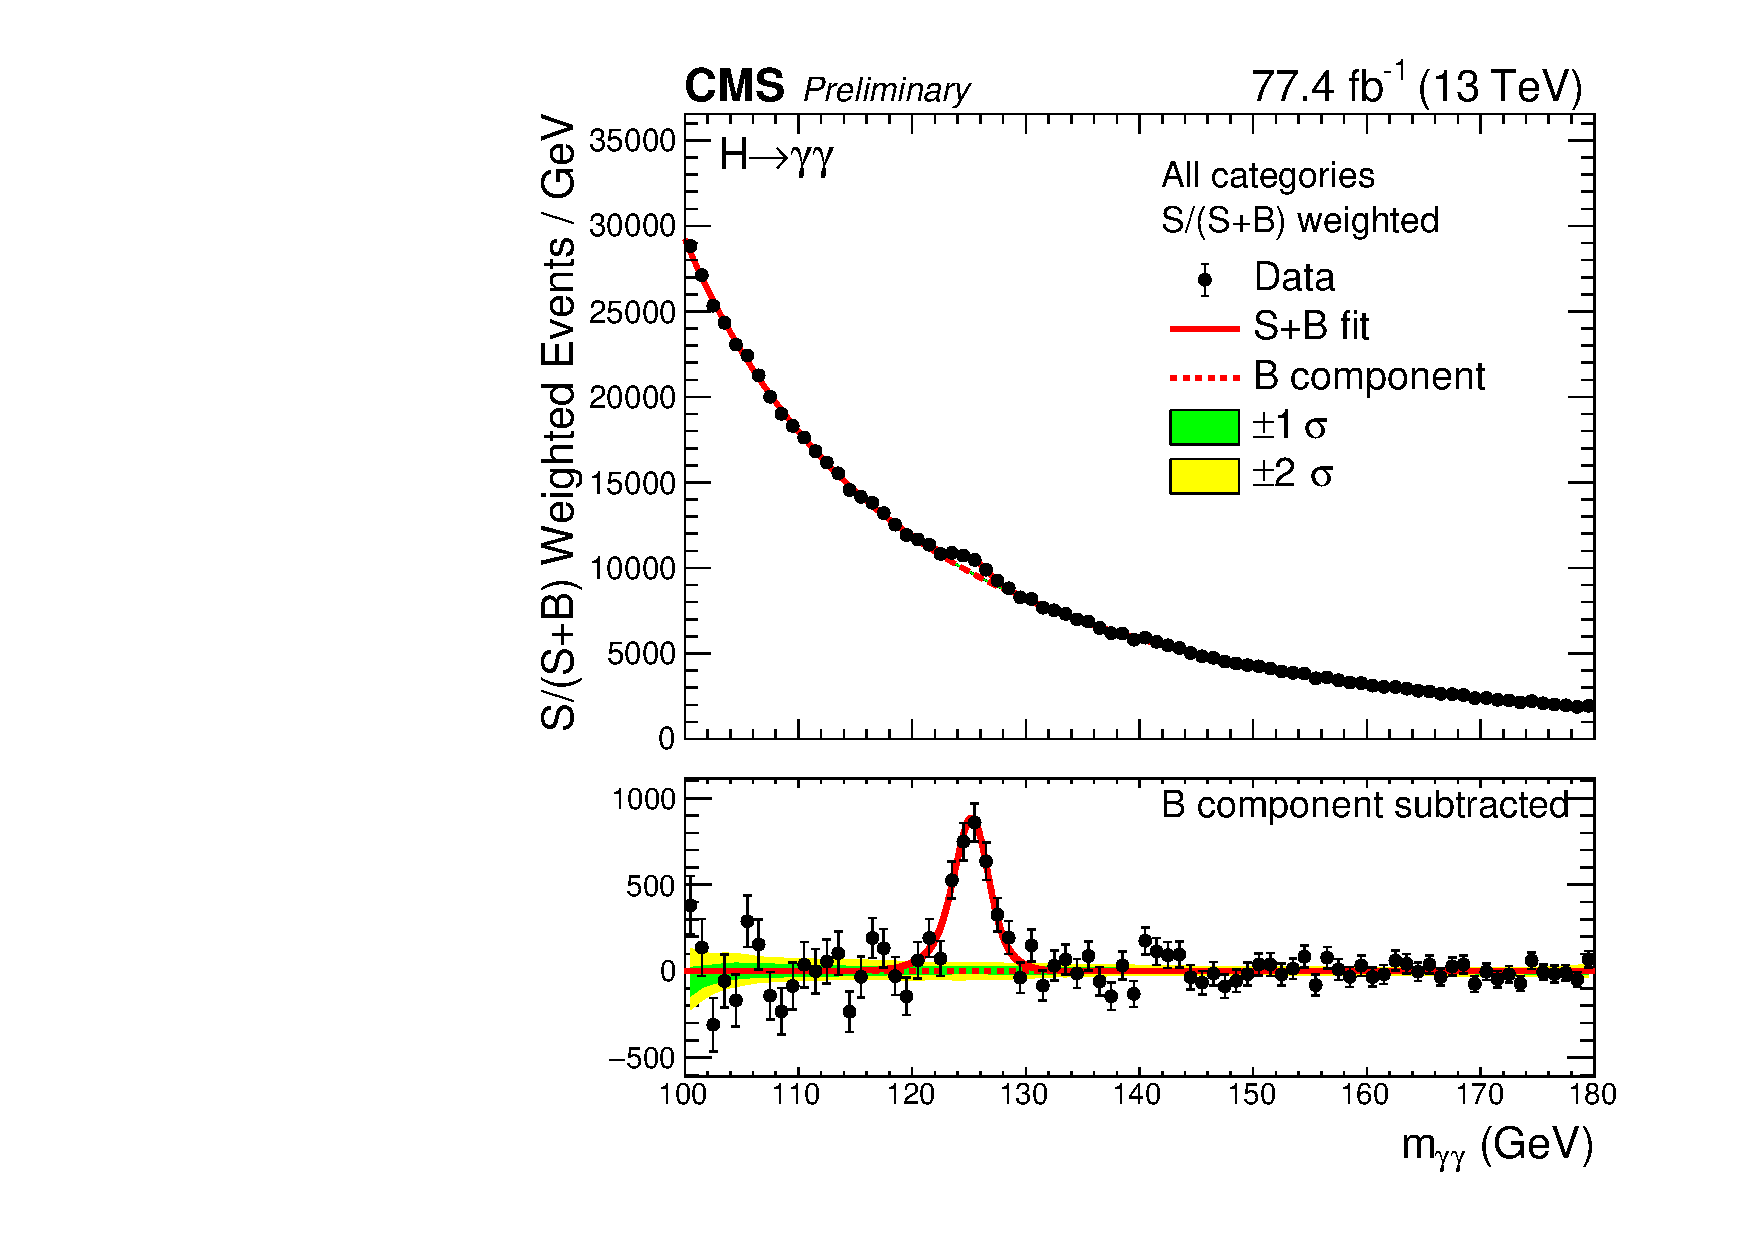
\includegraphics[width=\textwidth]{Figures/Results/MassPlot.pdf}
  \caption[Signal plus background fit to data, summed over all analysis categories.]
  {
    Data points (black) and signal plus background model fit 
    for the sum of all analysis categories is shown. 
    Each category is weighted by S/(S + B), 
    where S and B are the numbers of expected signal and background events, respectively, 
    in a $\pm 1 \seff$ mass window centred on \mH. 
    The one standard deviation (green) and two standard deviation (yellow) bands 
    include the uncertainties in the background component of the fit. 
    The solid red line shows the contribution from the total signal, plus the background contribution. 
    The dashed red line shows the contribution from the background component of the fit. 
    The bottom plot shows the residuals after subtraction of this background component.
    Figure first shown in Ref.~\cite{HIG-18-029}.
  }
  \label{fig:results_MassPlot}
\end{figure}

\begin{figure}[hptb]
  \centering
  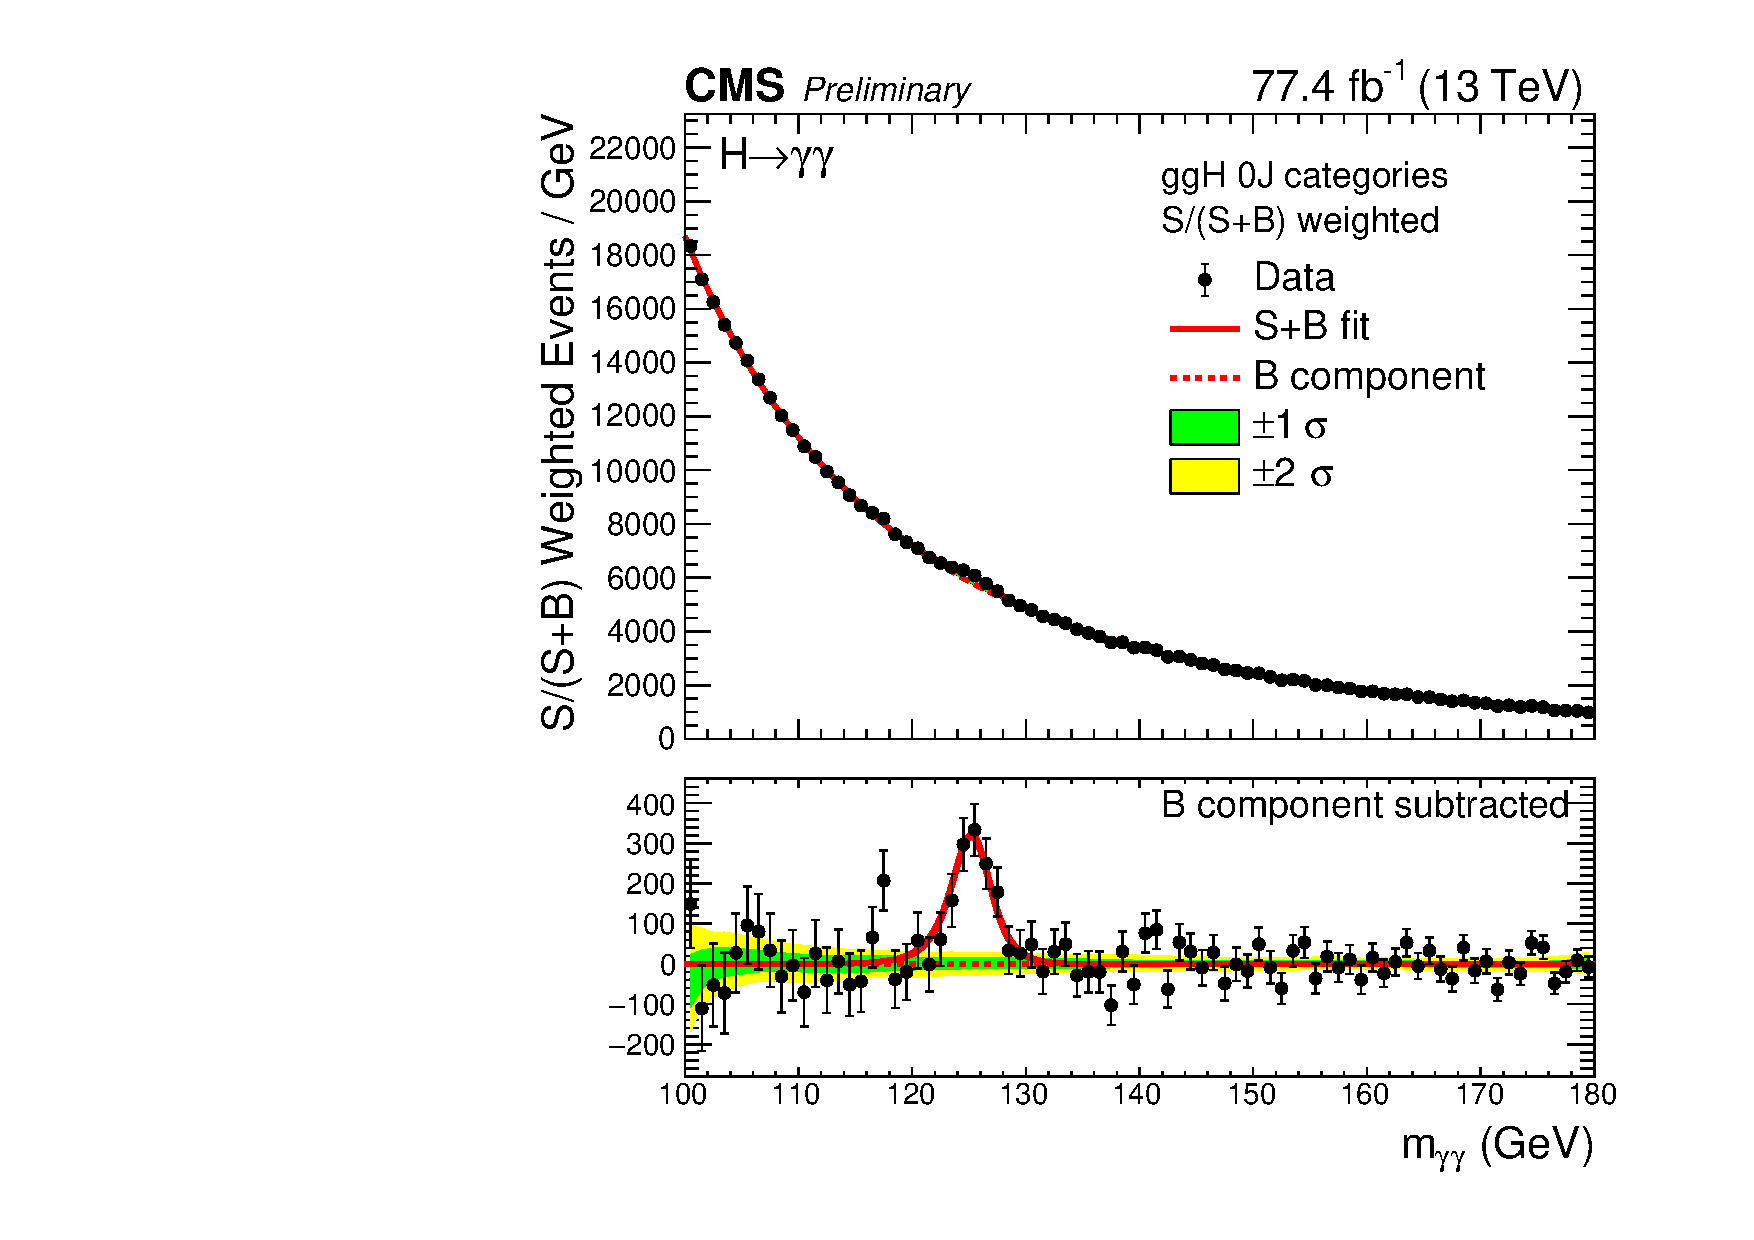
\includegraphics[width=0.49\textwidth]{Figures/Results/MassPlot_0J.pdf}
  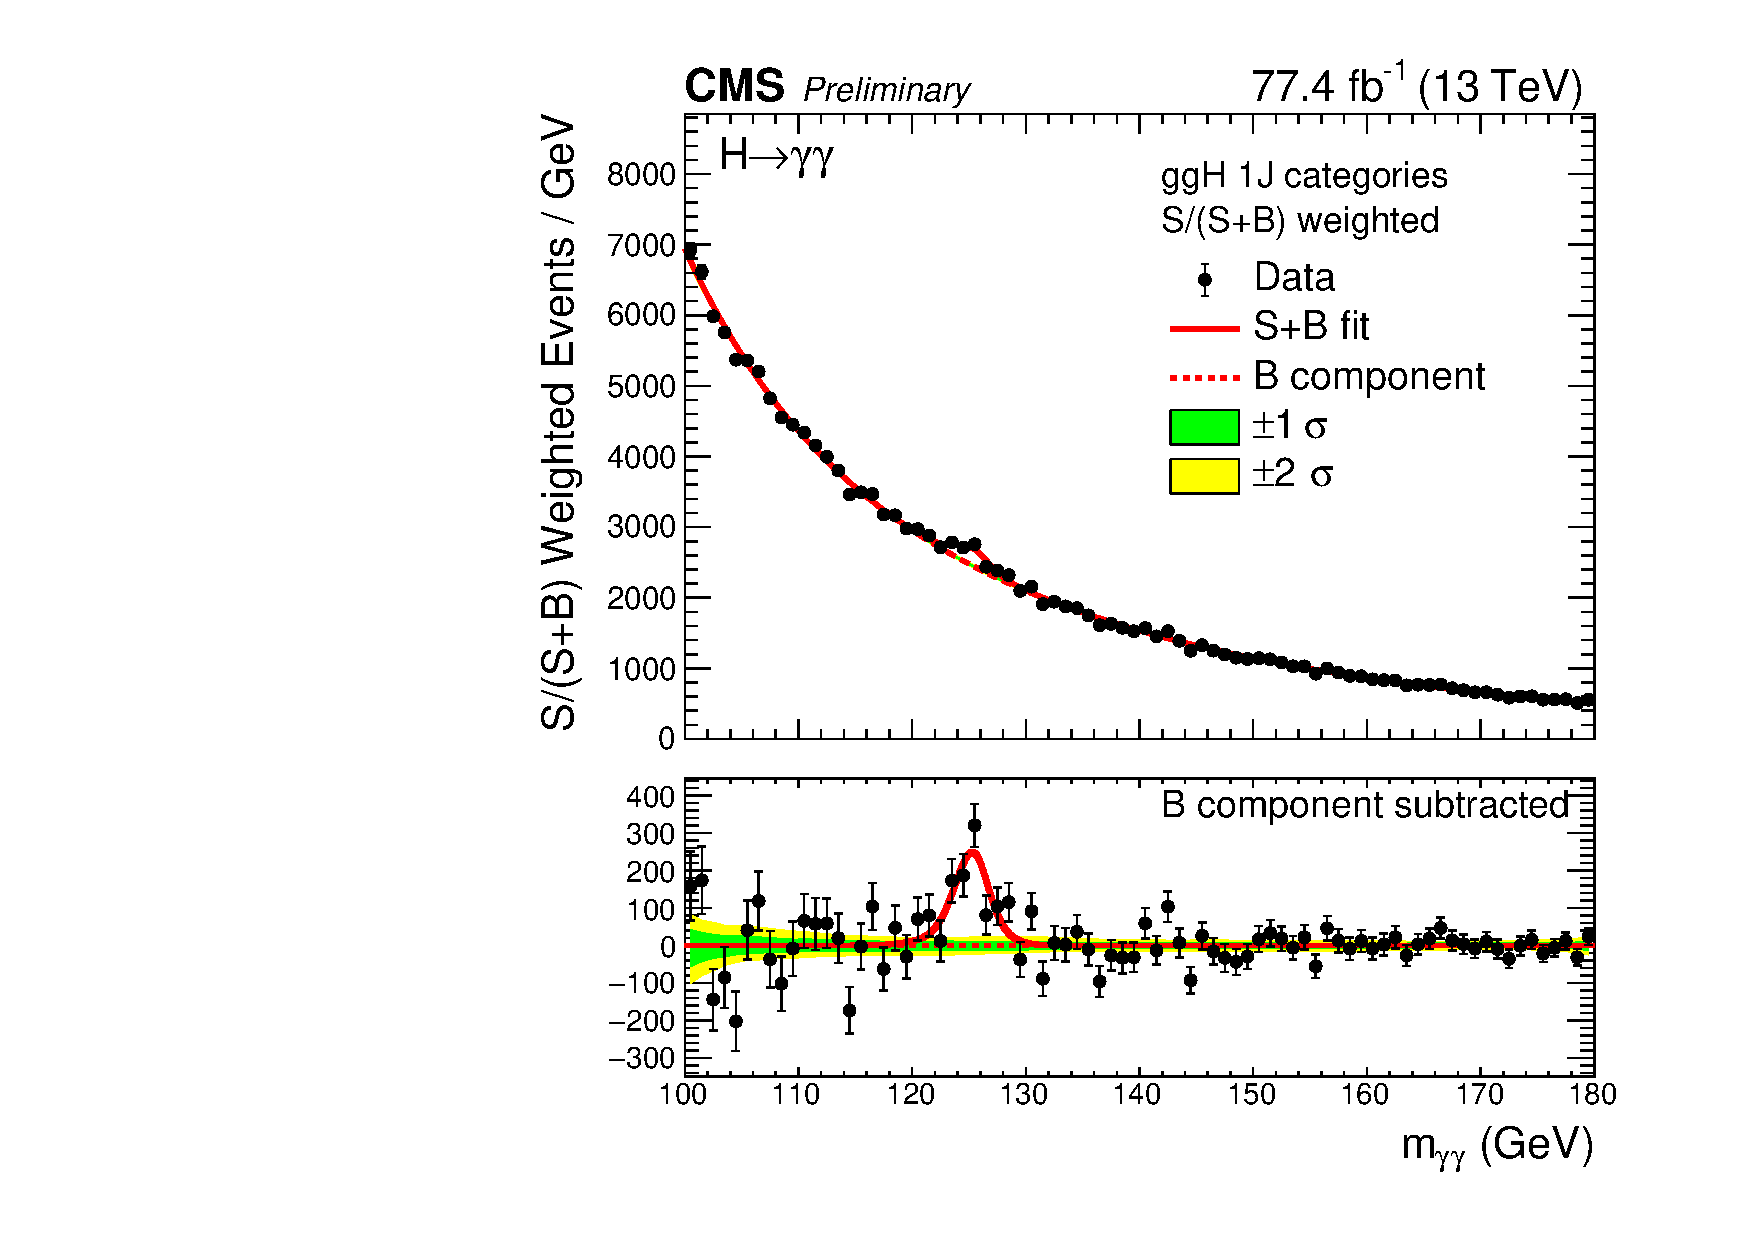
\includegraphics[width=0.49\textwidth]{Figures/Results/MassPlot_1J.pdf} \\
  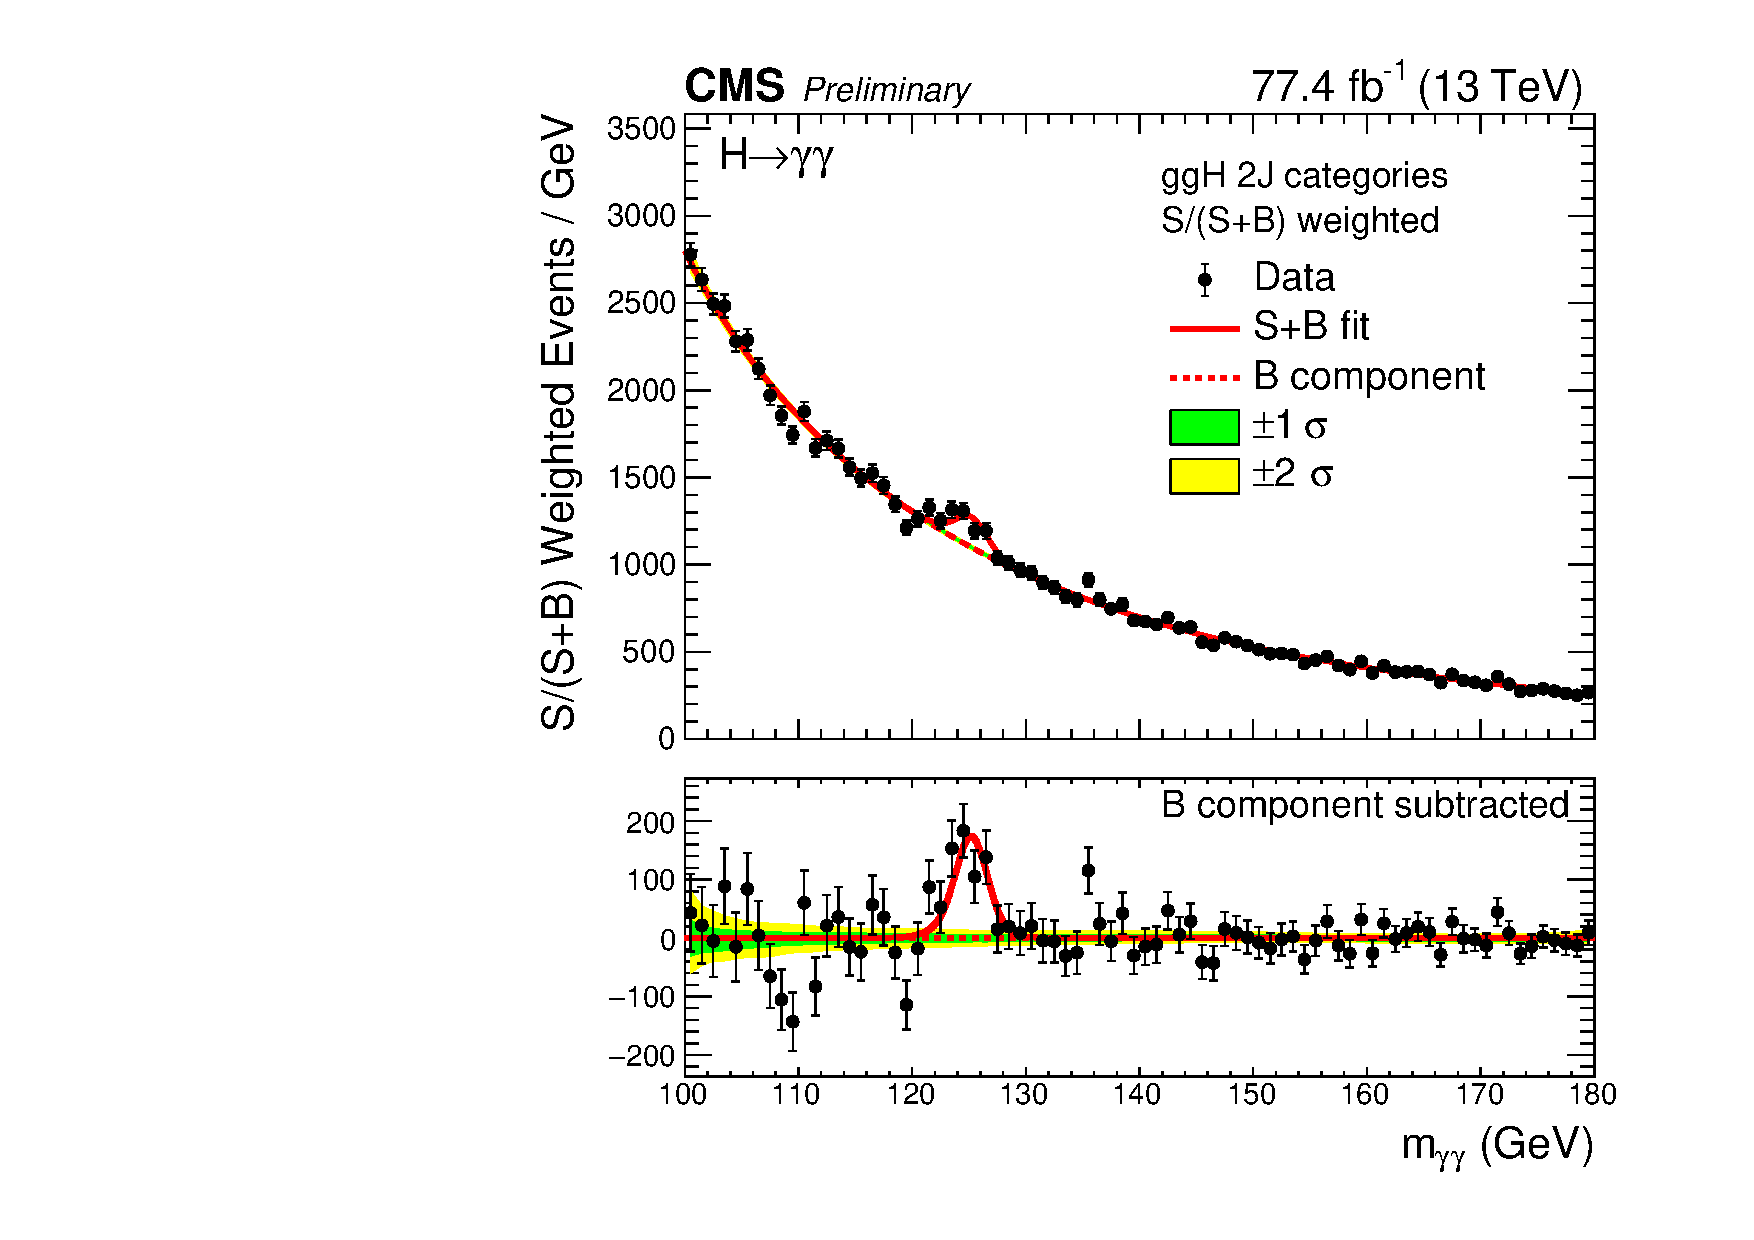
\includegraphics[width=0.49\textwidth]{Figures/Results/MassPlot_2J.pdf}
  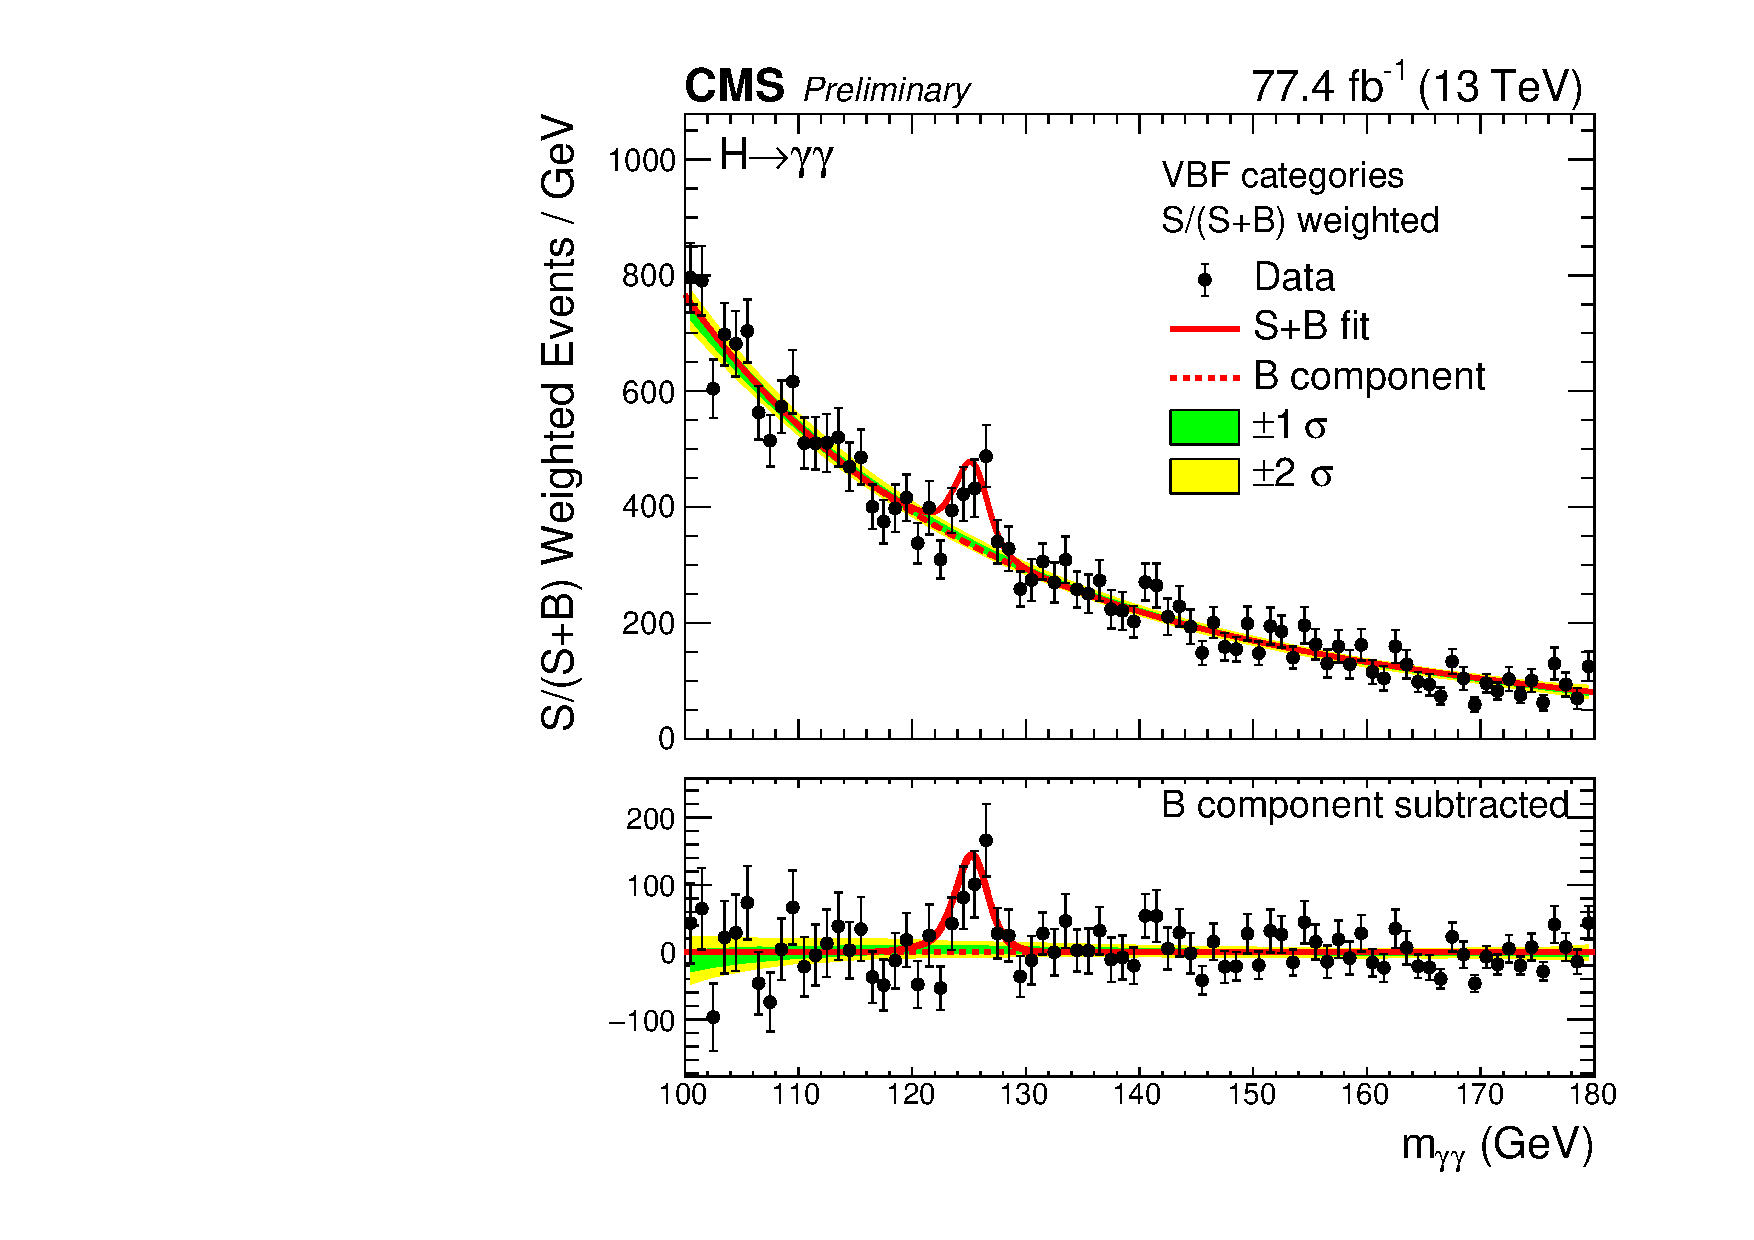
\includegraphics[width=0.49\textwidth]{Figures/Results/MassPlot_VBF.pdf}
  \caption[Signal plus background fits to data, 
           summed over analysis categories targeting different bins.]
  {
    Data points (black) and signal plus background model fit 
    for the ggH 0J, ggH 1J, ggH 2J, and VBF categories is shown. 
    Each category is weighted by S/(S + B), 
    where S and B are the numbers of expected signal and background events, respectively, 
    in a $\pm 1 \seff$ mass window centred on \mH. 
    The one standard deviation (green) and two standard deviation (yellow) bands 
    include the uncertainties in the background component of the fit. 
    The solid red line shows the contribution from the total signal, plus the background contribution. 
    The dashed red line shows the contribution from the background component of the fit. 
    The bottom plot shows the residuals after subtraction of this background component.
  }
  \label{fig:results_MassPlots}
\end{figure}

\section{Category composition}

All analysis categories are contaminated, to varying extents, 
by background events and other signal processes which are not being targeted.
The level of contamination then affects the sensitivity of the analysis 
when the final fits are performed.
Tables~\ref{tab:results_yields2016} and \ref{tab:results_yields2017} 
show the expected number of signal events for the 2016 and 2017 datasets respectively.
The relative contribution to each category from each of the individual stage 0 bins is shown, 
together with the \seff and \shm (the FWHM divided by 2.35) for the category's signal model.
Also reported is the expected number of background events per GeV in a $\pm1\seff$ window 
around \SI{125}{GeV}, calculated using the best-fit background function.
The table illustrates how the ratio of expected ratio of signal 
to signal plus background events (S/S+B) is highest in the ``Tag 0" categories, 
with lower S/S+B values but a greater number of events overall as the tag number increases.

The signal composition of the analysis categories in terms of the stage 1 bins being targeted
is shown in Figures~\ref{fig:results_Cats2016} and \ref{fig:results_Cats2017}.
The contribution of each bin to the total number of expected signal events in a category is displayed, 
meaning the values in each row sum to 100\%.
In general the migration between categories due to mis-measurement of \ptgg is very low, 
whilst there are significantly higher migrations arising from jet counting.

\begin{figure}[hptb]
  \centering
  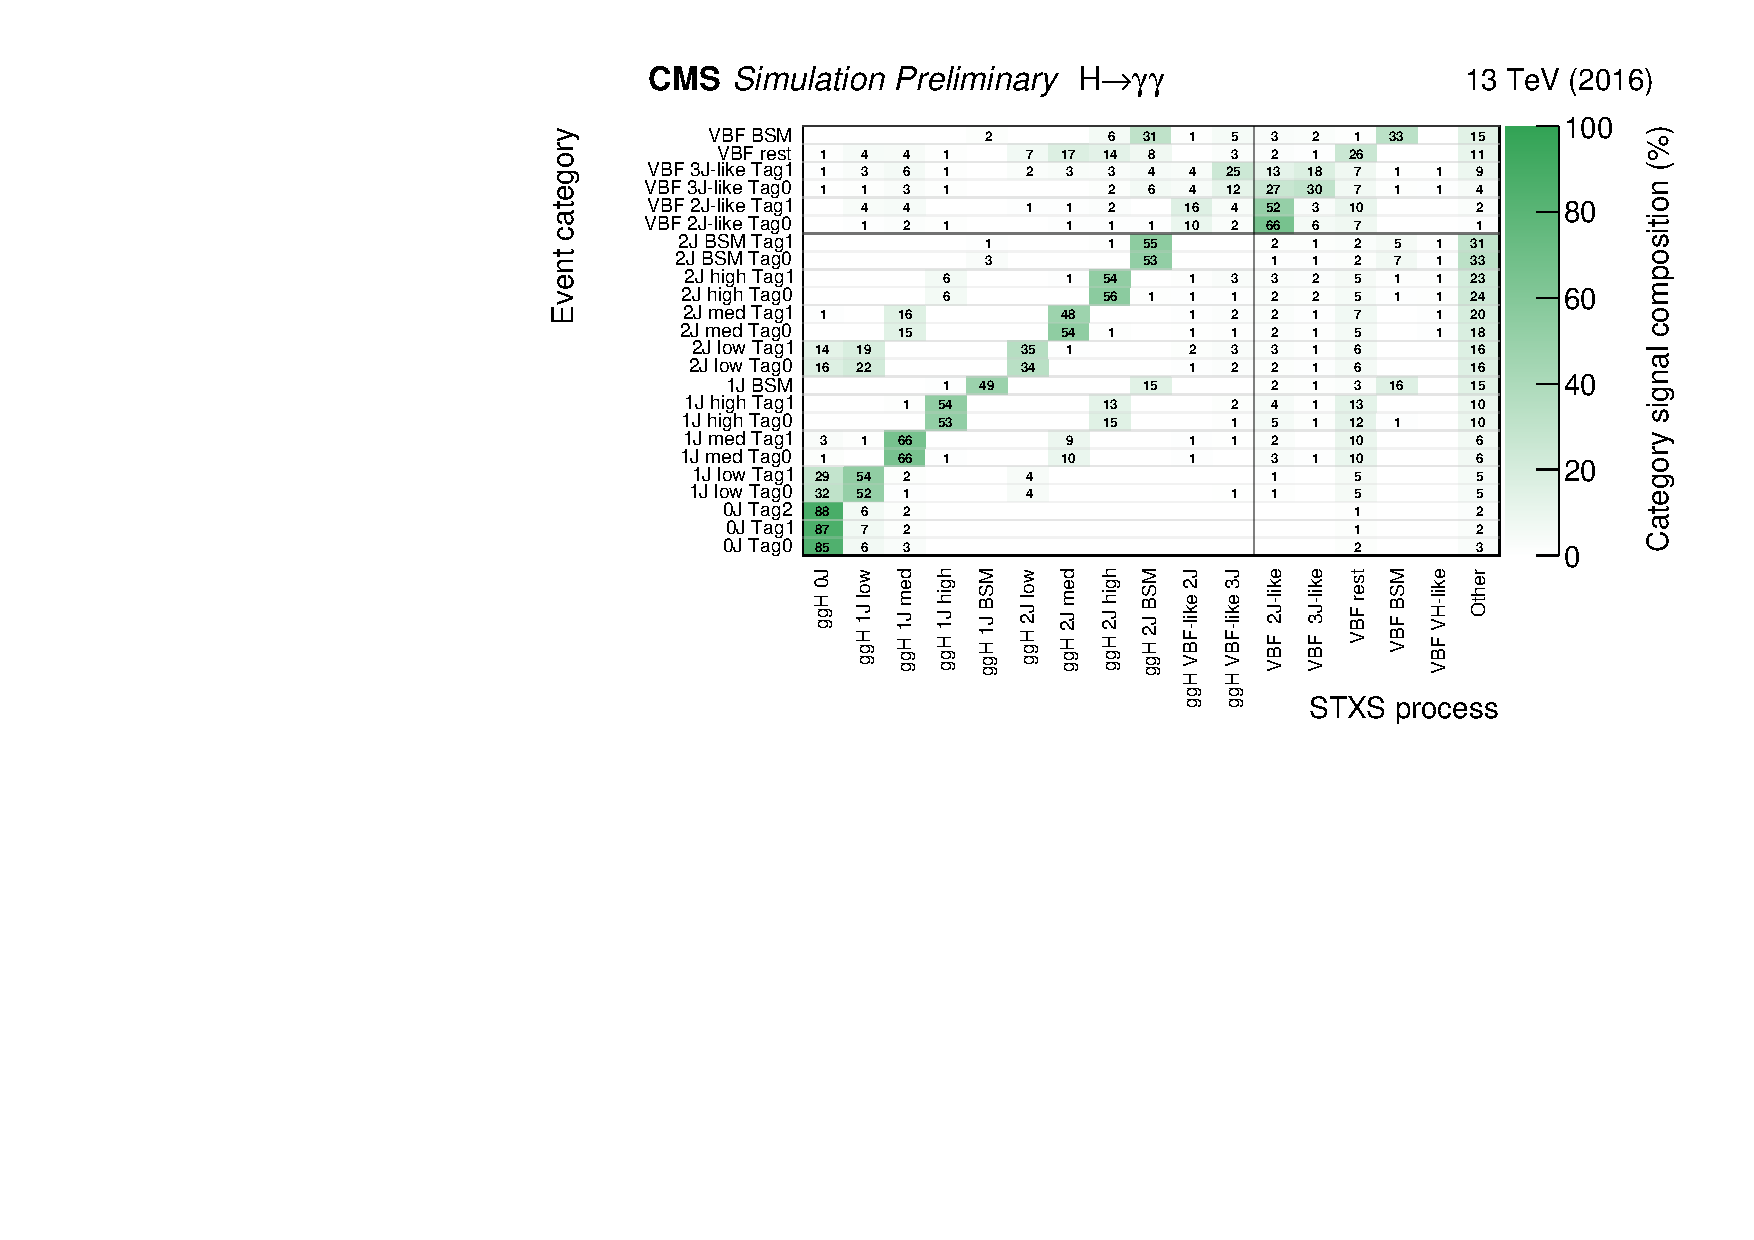
\includegraphics[width=\textwidth]{Figures/Results/Cats2016.pdf}
  \caption[Signal composition of 2016 analysis categories.]
  {
    The composition of each analysis category in terms of stage 1 bins is shown. 
    The colour scale corresponds to the fraction of each category (rows) 
    accounted for by each stage 1 process (columns). 
    Each row therefore sums to 100\%. 
    Entries with values less than 0.5\% are not shown. 
    Simulation corresponding to 2016 conditions is shown.
    Figure first shown in Ref.~\cite{HIG-18-029}.
  }
  \label{fig:results_Cats2016}
\end{figure}

\begin{figure}[hptb]
  \centering
  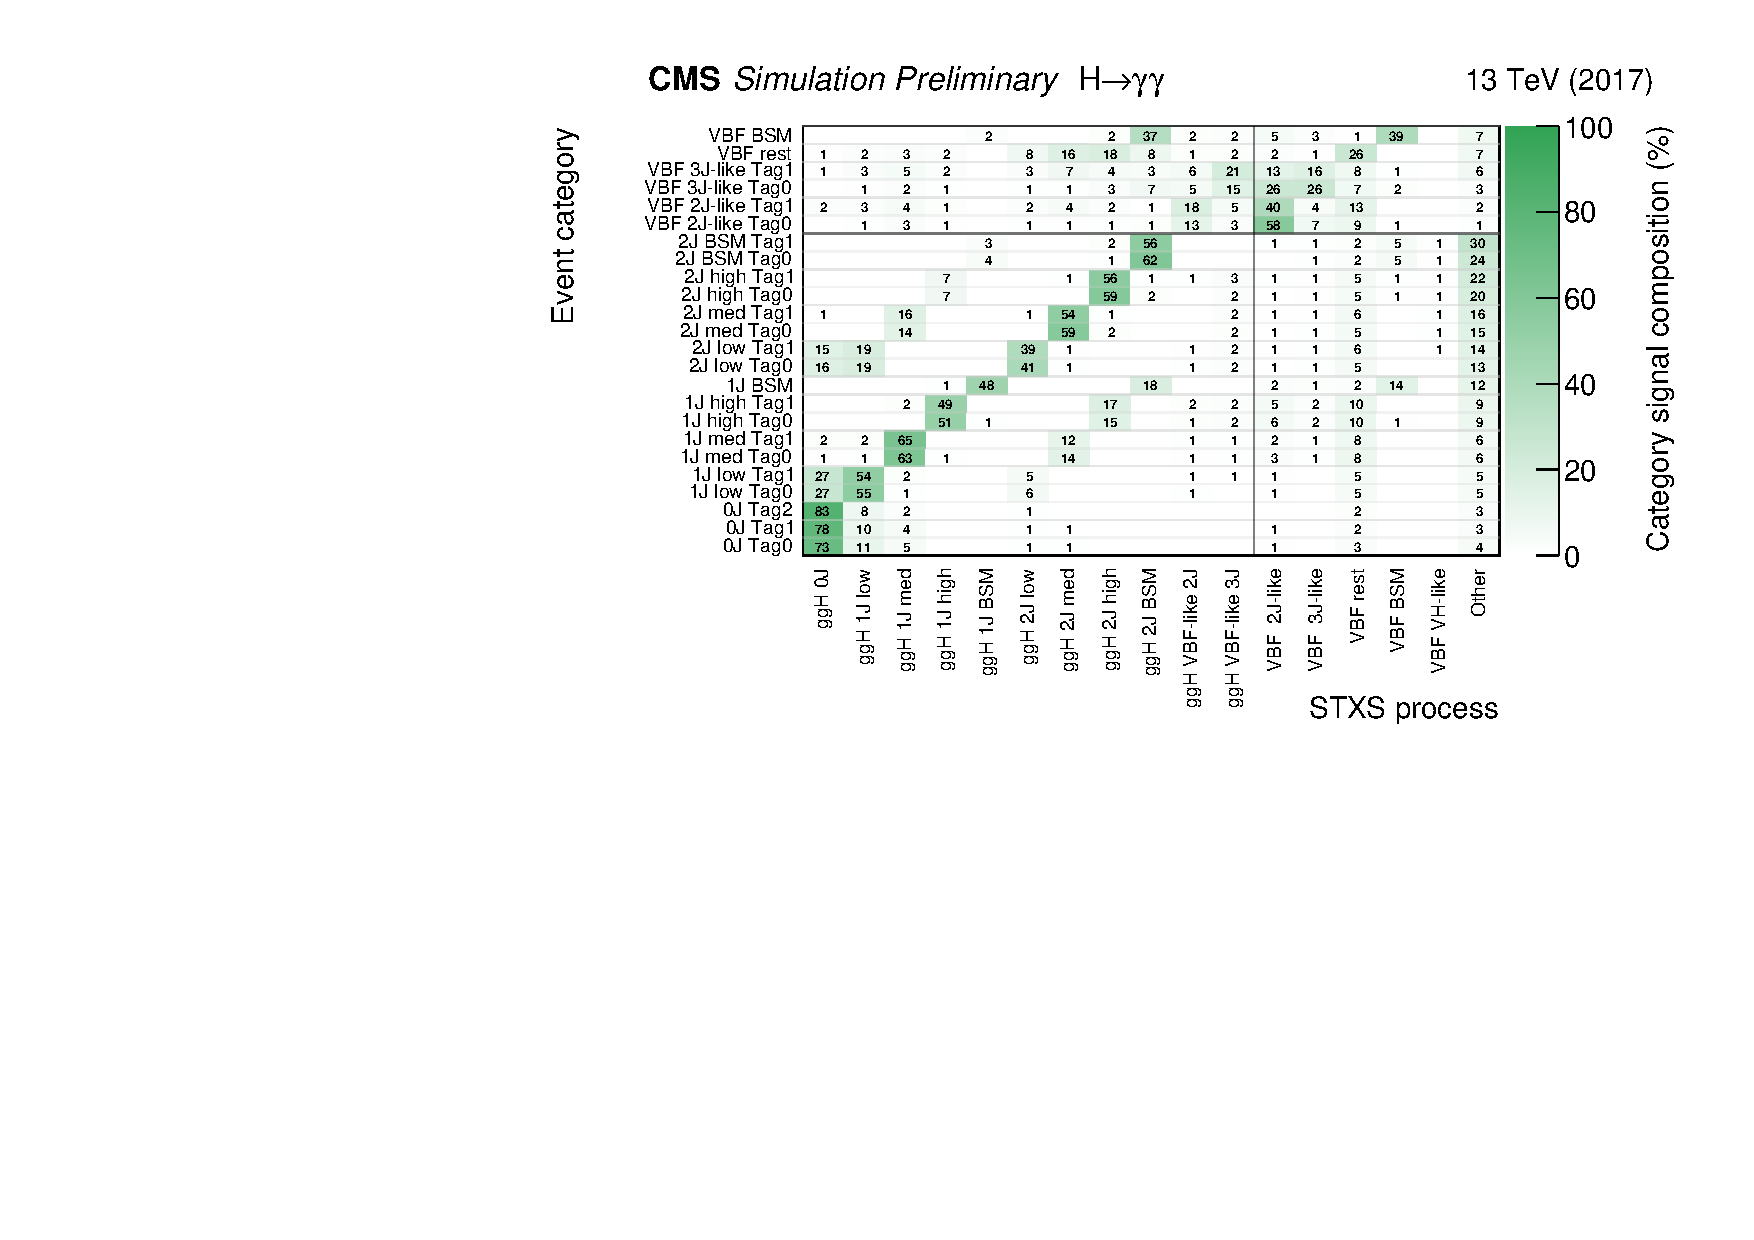
\includegraphics[width=\textwidth]{Figures/Results/Cats2017.pdf}
  \caption[Signal composition of 2017 analysis categories.]
  {
    The composition of each analysis category in terms of stage 1 bins is shown. 
    The colour scale corresponds to the fraction of each category (rows) 
    accounted for by each stage 1 process (columns). 
    Each row therefore sums to 100\%. 
    Entries with values less than 0.5\% are not shown. 
    Simulation corresponding to 2017 conditions is shown.
    Figure first shown in Ref.~\cite{HIG-18-029}.
  }
  \label{fig:results_Cats2017}
\end{figure}

\begin{landscape}
  \begin{table}
    \resizebox{1.5\textwidth}{!}{\begin{tabular}{ r | c | c | c  | c | c |  c |  c |  c |  c |  c |  c |  c |  c |  c |  c |  c }
\hline
\multirow{2}{*}{Event Categories} &\multicolumn{14}{|c|}{SM 125 GeV Higgs boson expected signal} & Bkg & S/(S+B) \\ \cline{2-15}
  &  Total & ggH & VBF & ttH & tHq & tHW & bbH & ggZH & WH lep & WH had & ZH lep & ZH had &   $\sigma_{eff} $  & $\sigma_{HM} $ & (GeV$^{-1}$) & \\ 
\hline
 0J Tag 0 &  257.1  &  95.0 \%  &  1.9 \%  &  $<$0.05 \%  &  $<$0.05 \%  &  $<$0.05 \%  &  0.9 \%  &  0.1 \%  &  0.9 \%  &  0.3 \%  &  0.7 \%  &  0.2 \%  & 1.66 & 1.48 & 522.7 & 0.09 \\
 0J Tag 1 &  356.4  &  96.0 \%  &  1.6 \%  &  $<$0.05 \%  &  $<$0.05 \%  &  $<$0.05 \%  &  0.9 \%  &  $<$0.05 \%  &  0.6 \%  &  0.4 \%  &  0.4 \%  &  0.2 \%  & 2.10 & 1.74 & 1182.2 & 0.05 \\
 0J Tag 2 &  417.2  &  96.5 \%  &  1.4 \%  &  $<$0.05 \%  &  $<$0.05 \%  &  $<$0.05 \%  &  0.8 \%  &  $<$0.05 \%  &  0.6 \%  &  0.3 \%  &  0.3 \%  &  0.2 \%  & 2.38 & 1.97 & 3229.8 & 0.02 \\
 1J Low Tag 0 &  115.1  &  88.9 \%  &  6.5 \%  &  0.1 \%  &  $<$0.05 \%  &  $<$0.05 \%  &  1.3 \%  &  $<$0.05 \%  &  0.6 \%  &  1.4 \%  &  0.2 \%  &  0.8 \%  & 1.61 & 1.37 & 269.6 & 0.08 \\
 1J Low Tag 1 &  145.5  &  89.2 \%  &  6.2 \%  &  0.1 \%  &  $<$0.05 \%  &  $<$0.05 \%  &  1.2 \%  &  $<$0.05 \%  &  0.6 \%  &  1.6 \%  &  0.3 \%  &  0.9 \%  & 2.13 & 1.82 & 722.3 & 0.03 \\
 1J Medium Tag 0 &  48.7  &  79.9 \%  &  13.7 \%  &  0.1 \%  &  0.1 \%  &  $<$0.05 \%  &  0.8 \%  &  0.3 \%  &  1.1 \%  &  2.2 \%  &  0.4 \%  &  1.4 \%  & 1.54 & 1.40 & 61.4 & 0.15 \\
 1J Medium Tag 1 &  109.1  &  81.1 \%  &  12.6 \%  &  0.1 \%  &  0.1 \%  &  $<$0.05 \%  &  0.9 \%  &  0.1 \%  &  1.0 \%  &  2.2 \%  &  0.5 \%  &  1.4 \%  & 1.86 & 1.61 & 383.9 & 0.05 \\
 1J High Tag 0 &  17.6  &  70.3 \%  &  19.8 \%  &  0.2 \%  &  0.1 \%  &  $<$0.05 \%  &  0.5 \%  &  0.7 \%  &  2.7 \%  &  2.9 \%  &  1.0 \%  &  1.7 \%  & 1.47 & 1.34 & 15.6 & 0.21 \\
 1J High Tag 1 &  21.2  &  70.8 \%  &  19.5 \%  &  0.3 \%  &  0.1 \%  &  $<$0.05 \%  &  0.4 \%  &  0.9 \%  &  2.5 \%  &  2.7 \%  &  1.1 \%  &  1.7 \%  & 1.74 & 1.64 & 61.3 & 0.06 \\
 1J BSM &  8.6  &  63.9 \%  &  21.6 \%  &  0.3 \%  &  0.2 \%  &  0.1 \%  &  0.3 \%  &  1.6 \%  &  4.9 \%  &  3.4 \%  &  2.0 \%  &  1.8 \%  & 1.40 & 1.35 & 6.0 & 0.26 \\
 2J Low Tag 0 &  28.8  &  75.7 \%  &  8.2 \%  &  4.2 \%  &  0.5 \%  &  $<$0.05 \%  &  3.0 \%  &  0.1 \%  &  0.9 \%  &  4.1 \%  &  0.5 \%  &  2.7 \%  & 1.61 & 1.21 & 86.2 & 0.07 \\
 2J Low Tag 1 &  38.5  &  73.3 \%  &  10.3 \%  &  4.2 \%  &  0.5 \%  &  $<$0.05 \%  &  2.7 \%  &  0.3 \%  &  0.9 \%  &  4.5 \%  &  0.5 \%  &  2.8 \%  & 1.98 & 1.70 & 254.7 & 0.03 \\
 2J Medium Tag 0 &  24.8  &  72.1 \%  &  9.6 \%  &  5.0 \%  &  0.6 \%  &  0.1 \%  &  1.7 \%  &  0.6 \%  &  0.8 \%  &  5.7 \%  &  0.5 \%  &  3.3 \%  & 1.50 & 1.36 & 38.7 & 0.13 \\
 2J Medium Tag 1 &  50.5  &  68.8 \%  &  11.2 \%  &  6.0 \%  &  0.6 \%  &  0.1 \%  &  2.1 \%  &  0.7 \%  &  0.9 \%  &  5.7 \%  &  0.5 \%  &  3.3 \%  & 1.85 & 1.54 & 213.2 & 0.04 \\
 2J High Tag 0 &  22.6  &  65.3 \%  &  11.2 \%  &  7.3 \%  &  1.0 \%  &  0.3 \%  &  0.9 \%  &  1.4 \%  &  1.4 \%  &  6.9 \%  &  0.5 \%  &  3.8 \%  & 1.52 & 1.41 & 21.7 & 0.19 \\
 2J High Tag 1 &  28.4  &  65.0 \%  &  11.9 \%  &  7.8 \%  &  0.9 \%  &  0.2 \%  &  1.0 \%  &  1.7 \%  &  1.1 \%  &  6.4 \%  &  0.5 \%  &  3.6 \%  & 1.78 & 1.72 & 79.8 & 0.06 \\
 2J BSM Tag 0 &  14.6  &  56.3 \%  &  11.1 \%  &  11.5 \%  &  1.9 \%  &  1.2 \%  &  0.3 \%  &  2.6 \%  &  1.5 \%  &  8.1 \%  &  0.7 \%  &  4.9 \%  & 1.40 & 1.33 & 6.5 & 0.35 \\
 2J BSM Tag 1 &  9.7  &  57.8 \%  &  11.5 \%  &  12.1 \%  &  1.6 \%  &  0.9 \%  &  0.4 \%  &  1.4 \%  &  1.6 \%  &  7.7 \%  &  0.7 \%  &  4.2 \%  & 1.64 & 1.53 & 17.3 & 0.10 \\
 VBF 2J-like Tag 0 &  12.9  &  19.5 \%  &  79.8 \%  &  0.1 \%  &  0.1 \%  &  $<$0.05 \%  &  0.3 \%  &  0.1 \%  &  0.1 \%  &  0.1 \%  &  $<$0.05 \%  &  $<$0.05 \%  & 1.70 & 1.41 & 4.9 & 0.35 \\
 VBF 2J-like Tag 1 &  6.2  &  32.4 \%  &  65.5 \%  &  0.3 \%  &  0.2 \%  &  $<$0.05 \%  &  0.7 \%  &  0.1 \%  &  0.2 \%  &  0.5 \%  &  $<$0.05 \%  &  0.1 \%  & 1.85 & 1.52 & 8.4 & 0.12 \\
 VBF 3J-like Tag 0 &  12.0  &  30.6 \%  &  65.6 \%  &  1.3 \%  &  0.7 \%  &  0.1 \%  &  0.8 \%  &  0.4 \%  &  0.1 \%  &  0.3 \%  &  $<$0.05 \%  &  0.2 \%  & 1.59 & 1.34 & 6.0 & 0.30 \\
 VBF 3J-like Tag 1 &  13.6  &  52.5 \%  &  38.9 \%  &  3.2 \%  &  1.2 \%  &  0.1 \%  &  1.1 \%  &  0.4 \%  &  0.5 \%  &  1.1 \%  &  0.3 \%  &  0.7 \%  & 1.71 & 1.51 & 19.5 & 0.12 \\
 VBF Rest &  13.0  &  59.5 \%  &  29.4 \%  &  3.5 \%  &  1.0 \%  &  0.2 \%  &  1.4 \%  &  0.7 \%  &  1.0 \%  &  2.0 \%  &  0.3 \%  &  1.0 \%  & 1.50 & 1.29 & 21.2 & 0.12 \\
 VBF BSM &  7.2  &  45.5 \%  &  39.9 \%  &  6.5 \%  &  1.0 \%  &  0.8 \%  &  0.9 \%  &  1.1 \%  &  1.0 \%  &  2.2 \%  &  0.1 \%  &  1.0 \%  & 1.48 & 1.29 & 6.0 & 0.22 \\
Total &    1779.2  &  87.5 \%  &  6.7 \%  &  0.9 \%  &  0.1 \%  &  $<$0.05 \%  &  1.0 \%  &  0.2 \%  &  0.8 \%  &  1.4 \%  &  0.4 \%  &  0.8 \%  & 1.96 & 1.67 & 7238.9 & 0.04 \\
\hline
\end{tabular}
}
    \caption[Signal and background yields for 2016 analysis categories.]
    {
      The expected number of signal events per category and
      the percentage breakdown per production mode in that category. 
      The $\sigma_{eff}$, computed as the smallest interval containing 68.3\% 
      of the invariant mass distribution, and $\sigma_{HM}$, computed as the FWHM divided by 2.35,
      are also shown as an estimate of the \mgg resolution in that category.
      The expected number of background events per GeV around 125 GeV is listed.
      The expected ratio of signal to signal plus background events, S/(S + B), is also shown,
      where S and B are the numbers of expected signal and background events, respectively, 
      in a $\pm 1 \sigma_{eff}$ mass window centred on \mH.
      Data and simulation from 2016 are shown.
    }
    \label{tab:results_yields2016}
  \end{table}
\end{landscape}

\begin{landscape}
  \begin{table}
    \resizebox{1.5\textwidth}{!}{\begin{tabular}{ r | c | c | c  | c | c |  c |  c |  c |  c |  c |  c |  c |  c |  c |  c |  c }
\hline
\multirow{2}{*}{Event Categories} &\multicolumn{14}{|c|}{SM 125 GeV Higgs boson expected signal} & Bkg & S/(S+B) \\ \cline{2-15}
  &  Total & ggH & VBF & ttH & tHq & tHW & bbH & ggZH & WH lep & WH had & ZH lep & ZH had &   $\sigma_{eff} $  & $\sigma_{HM} $ & (GeV$^{-1}$) & \\ 
\hline
 0J Tag 0 &  401.1  &  91.8 \%  &  4.4 \%  &  $<$0.05 \%  &  $<$0.05 \%  &  $<$0.05 \%  &  1.4 \%  &  0.1 \%  &  1.0 \%  &  0.4 \%  &  0.6 \%  &  0.2 \%  & 1.94 & 1.79 & 870.3 & 0.07 \\
 0J Tag 1 &  552.3  &  93.7 \%  &  3.1 \%  &  $<$0.05 \%  &  $<$0.05 \%  &  $<$0.05 \%  &  1.3 \%  &  $<$0.05 \%  &  0.7 \%  &  0.4 \%  &  0.4 \%  &  0.2 \%  & 2.42 & 2.06 & 2121.9 & 0.04 \\
 0J Tag 2 &  347.3  &  95.0 \%  &  2.2 \%  &  $<$0.05 \%  &  $<$0.05 \%  &  $<$0.05 \%  &  1.3 \%  &  $<$0.05 \%  &  0.5 \%  &  0.4 \%  &  0.3 \%  &  0.2 \%  & 2.72 & 2.41 & 3035.8 & 0.01 \\
 1J Low Tag 0 &  130.8  &  89.5 \%  &  5.9 \%  &  0.1 \%  &  $<$0.05 \%  &  $<$0.05 \%  &  1.1 \%  &  $<$0.05 \%  &  0.5 \%  &  1.7 \%  &  0.2 \%  &  0.9 \%  & 1.91 & 1.71 & 360.2 & 0.06 \\
 1J Low Tag 1 &  111.5  &  89.2 \%  &  6.1 \%  &  0.1 \%  &  $<$0.05 \%  &  $<$0.05 \%  &  1.1 \%  &  $<$0.05 \%  &  0.5 \%  &  1.8 \%  &  0.2 \%  &  1.0 \%  & 2.47 & 2.22 & 689.4 & 0.02 \\
 1J Medium Tag 0 &  71.4  &  81.5 \%  &  12.4 \%  &  0.2 \%  &  0.1 \%  &  $<$0.05 \%  &  0.5 \%  &  0.2 \%  &  0.9 \%  &  2.5 \%  &  0.4 \%  &  1.3 \%  & 1.85 & 1.67 & 110.8 & 0.11 \\
 1J Medium Tag 1 &  91.1  &  82.7 \%  &  11.4 \%  &  0.2 \%  &  0.1 \%  &  $<$0.05 \%  &  0.5 \%  &  0.2 \%  &  0.8 \%  &  2.3 \%  &  0.4 \%  &  1.4 \%  & 2.13 & 1.91 & 342.2 & 0.04 \\
 1J High Tag 0 &  14.7  &  71.7 \%  &  19.4 \%  &  0.3 \%  &  0.2 \%  &  $<$0.05 \%  &  0.3 \%  &  1.0 \%  &  2.3 \%  &  2.5 \%  &  1.0 \%  &  1.5 \%  & 1.54 & 1.51 & 8.7 & 0.27 \\
 1J High Tag 1 &  28.2  &  72.4 \%  &  18.4 \%  &  0.4 \%  &  0.2 \%  &  $<$0.05 \%  &  0.3 \%  &  0.8 \%  &  2.2 \%  &  2.8 \%  &  0.9 \%  &  1.7 \%  & 1.76 & 1.77 & 47.7 & 0.10 \\
 1J BSM &  15.5  &  66.9 \%  &  20.9 \%  &  0.4 \%  &  0.3 \%  &  0.1 \%  &  0.1 \%  &  1.0 \%  &  4.0 \%  &  3.0 \%  &  1.6 \%  &  1.8 \%  & 1.76 & 1.71 & 17.5 & 0.15 \\
 2J Low Tag 0 &  10.9  &  80.2 \%  &  7.0 \%  &  1.7 \%  &  0.4 \%  &  $<$0.05 \%  &  1.0 \%  &  0.3 \%  &  0.7 \%  &  4.8 \%  &  0.3 \%  &  3.4 \%  & 1.55 & 1.52 & 35.1 & 0.06 \\
 2J Low Tag 1 &  40.8  &  77.6 \%  &  8.1 \%  &  3.0 \%  &  0.5 \%  &  $<$0.05 \%  &  0.8 \%  &  0.3 \%  &  0.7 \%  &  5.4 \%  &  0.3 \%  &  3.1 \%  & 2.06 & 1.94 & 249.0 & 0.03 \\
 2J Medium Tag 0 &  16.8  &  76.6 \%  &  8.1 \%  &  1.9 \%  &  0.5 \%  &  0.1 \%  &  0.3 \%  &  1.0 \%  &  0.7 \%  &  7.0 \%  &  0.4 \%  &  3.4 \%  & 1.60 & 1.46 & 28.9 & 0.11 \\
 2J Medium Tag 1 &  49.7  &  74.6 \%  &  9.1 \%  &  3.4 \%  &  0.6 \%  &  0.1 \%  &  0.4 \%  &  0.8 \%  &  0.9 \%  &  6.1 \%  &  0.4 \%  &  3.6 \%  & 2.12 & 1.86 & 228.8 & 0.03 \\
 2J High Tag 0 &  14.0  &  71.1 \%  &  9.2 \%  &  1.7 \%  &  0.6 \%  &  0.1 \%  &  0.2 \%  &  2.7 \%  &  1.0 \%  &  8.2 \%  &  0.7 \%  &  4.6 \%  & 1.54 & 1.52 & 14.2 & 0.18 \\
 2J High Tag 1 &  24.4  &  69.1 \%  &  9.4 \%  &  3.7 \%  &  0.8 \%  &  0.2 \%  &  0.2 \%  &  2.3 \%  &  1.1 \%  &  8.2 \%  &  0.5 \%  &  4.7 \%  & 1.42 & 1.31 & 64.4 & 0.08 \\
 2J BSM Tag 0 &  15.8  &  66.4 \%  &  9.4 \%  &  2.6 \%  &  0.9 \%  &  0.4 \%  &  0.1 \%  &  2.7 \%  &  1.9 \%  &  9.3 \%  &  0.9 \%  &  5.4 \%  & 1.67 & 1.63 & 11.1 & 0.22 \\
 2J BSM Tag 1 &  5.7  &  60.4 \%  &  9.5 \%  &  9.2 \%  &  1.4 \%  &  0.7 \%  &  0.1 \%  &  2.7 \%  &  1.4 \%  &  9.0 \%  &  1.0 \%  &  4.7 \%  & 1.89 & 1.82 & 24.3 & 0.04 \\
 VBF 2J-like Tag 0 &  13.5  &  24.8 \%  &  74.4 \%  &  0.1 \%  &  0.1 \%  &  $<$0.05 \%  &  0.1 \%  &  0.1 \%  &  $<$0.05 \%  &  0.2 \%  &  $<$0.05 \%  &  0.2 \%  & 1.90 & 1.73 & 5.7 & 0.30 \\
 VBF 2J-like Tag 1 &  4.8  &  41.7 \%  &  56.5 \%  &  0.2 \%  &  0.2 \%  &  $<$0.05 \%  &  0.2 \%  &  0.2 \%  &  0.2 \%  &  0.5 \%  &  $<$0.05 \%  &  0.3 \%  & 2.28 & 1.94 & 9.3 & 0.07 \\
 VBF 3J-like Tag 0 &  12.7  &  36.8 \%  &  60.6 \%  &  0.4 \%  &  0.5 \%  &  $<$0.05 \%  &  0.1 \%  &  0.4 \%  &  0.2 \%  &  0.5 \%  &  0.1 \%  &  0.2 \%  & 1.90 & 1.69 & 7.8 & 0.23 \\
 VBF 3J-like Tag 1 &  7.6  &  56.0 \%  &  37.8 \%  &  0.8 \%  &  0.9 \%  &  $<$0.05 \%  &  0.2 \%  &  0.8 \%  &  0.5 \%  &  1.6 \%  &  0.2 \%  &  1.0 \%  & 1.86 & 1.79 & 11.1 & 0.11 \\
 VBF Rest &  12.9  &  63.4 \%  &  29.9 \%  &  1.0 \%  &  0.6 \%  &  0.1 \%  &  0.4 \%  &  0.8 \%  &  0.6 \%  &  2.0 \%  &  0.3 \%  &  1.1 \%  & 1.80 & 1.71 & 21.3 & 0.10 \\
 VBF BSM &  6.5  &  44.7 \%  &  47.8 \%  &  1.0 \%  &  0.5 \%  &  0.3 \%  &  0.1 \%  &  1.4 \%  &  0.7 \%  &  2.1 \%  &  0.4 \%  &  1.0 \%  & 1.75 & 1.45 & 4.5 & 0.22 \\
Total &    1999.8  &  88.2 \%  &  6.7 \%  &  0.4 \%  &  0.1 \%  &  $<$0.05 \%  &  1.1 \%  &  0.2 \%  &  0.8 \%  &  1.4 \%  &  0.4 \%  &  0.8 \%  & 2.22 & 1.98 & 8320.2 & 0.04 \\
\hline
\end{tabular}
}
    \caption[Signal and background yields for 2017 analysis categories.]
    {
      The expected number of signal events per category and
      the percentage breakdown per production mode in that category. 
      The $\sigma_{eff}$, computed as the smallest interval containing 68.3\% 
      of the invariant mass distribution, and $\sigma_{HM}$, computed as the FWHM divided by 2.35,
      are also shown as an estimate of the \mgg resolution in that category.
      The expected number of background events per GeV around 125 GeV is listed.
      The expected ratio of signal to signal plus background events, S/(S + B), is also shown,
      where S and B are the numbers of expected signal and background events, respectively, 
      in a $\pm 1 \sigma_{eff}$ mass window centred on \mH.
      Data and simulation from 2017 are shown.
    }
    \label{tab:results_yields2017}
  \end{table}
\end{landscape}

\section{Results in the STXS framework}

Results in the STXS framework are presented with three different parameterisations;
for each result the underlying signal bins 
are grouped into different parameters which are free to vary in the fit.
The recommendations contained in Ref.~\cite{YR4} 
concerning how to treat sub-dominant processes are followed in each case.
The ggH parameters include bbH events.
The ggZH process is grouped together with leptonic VH production if the Z boson decays leptonically, 
and with ggH otherwise.
The hadronic VH processes are grouped with VBF production to form the qqH parameters.
In each fit, the ttH, tH, and VH leptonic parameters are constrained to their SM prediction. 
This is necessary since there are no categories targeting these production modes, 
and therefore the parameters would be almost unconstrained 
and cause increased uncertainties in the other parameters of interest.
In all fits the mass of the Higgs boson is profiled.

\subsection{Stage 0 cross sections}
Measurements of stage 0 STXS bins are performed in a fit with two parameters, ggH and qqH.
The resulting cross sections, normalised to the SM prediction, are found to be 
%$\sigma_{ggH}/\sigma_{ggH}^{\textrm{SM}} = 1.00 \pm 0.13$ 
%and $\sigma_{qqH}^{\textrm{SM}} = 1.0 \pm 0.4$.
$\sigma_{ggH}/\sigma_{ggH}^{\textrm{SM}} = 1.15_{-0.15}^{+0.15}$ 
and $\sigma_{qqH}/\sigma_{qqH}^{\textrm{SM}} = 0.83_{-0.31}^{+0.37}$.
The individual likelihood scans are shown 
in Figures~\ref{fig:results_Stage0_ggH} and \ref{fig:results_Stage0_qqH}.
Two scans are shown, one corresponding to the full fit
and one corresponding to the fit without systematic uncertainties.
The systematic component of the uncertainty is then determined 
by subtracting the statistical component from the total uncertainty.
In both measurements the statistical component of the uncertainty 
is greater than the systematic component.
However for the ggH cross section, the magnitude of each is comparable.
With the full Run 2 dataset, 
which will increase the available integrated luminosity to around \SI{137}{\fbinv}, 
the ggH measurement is likely to become systematics-dominated.

%TODO add a 2D scan? 

\begin{figure}[hptb]
  \centering
  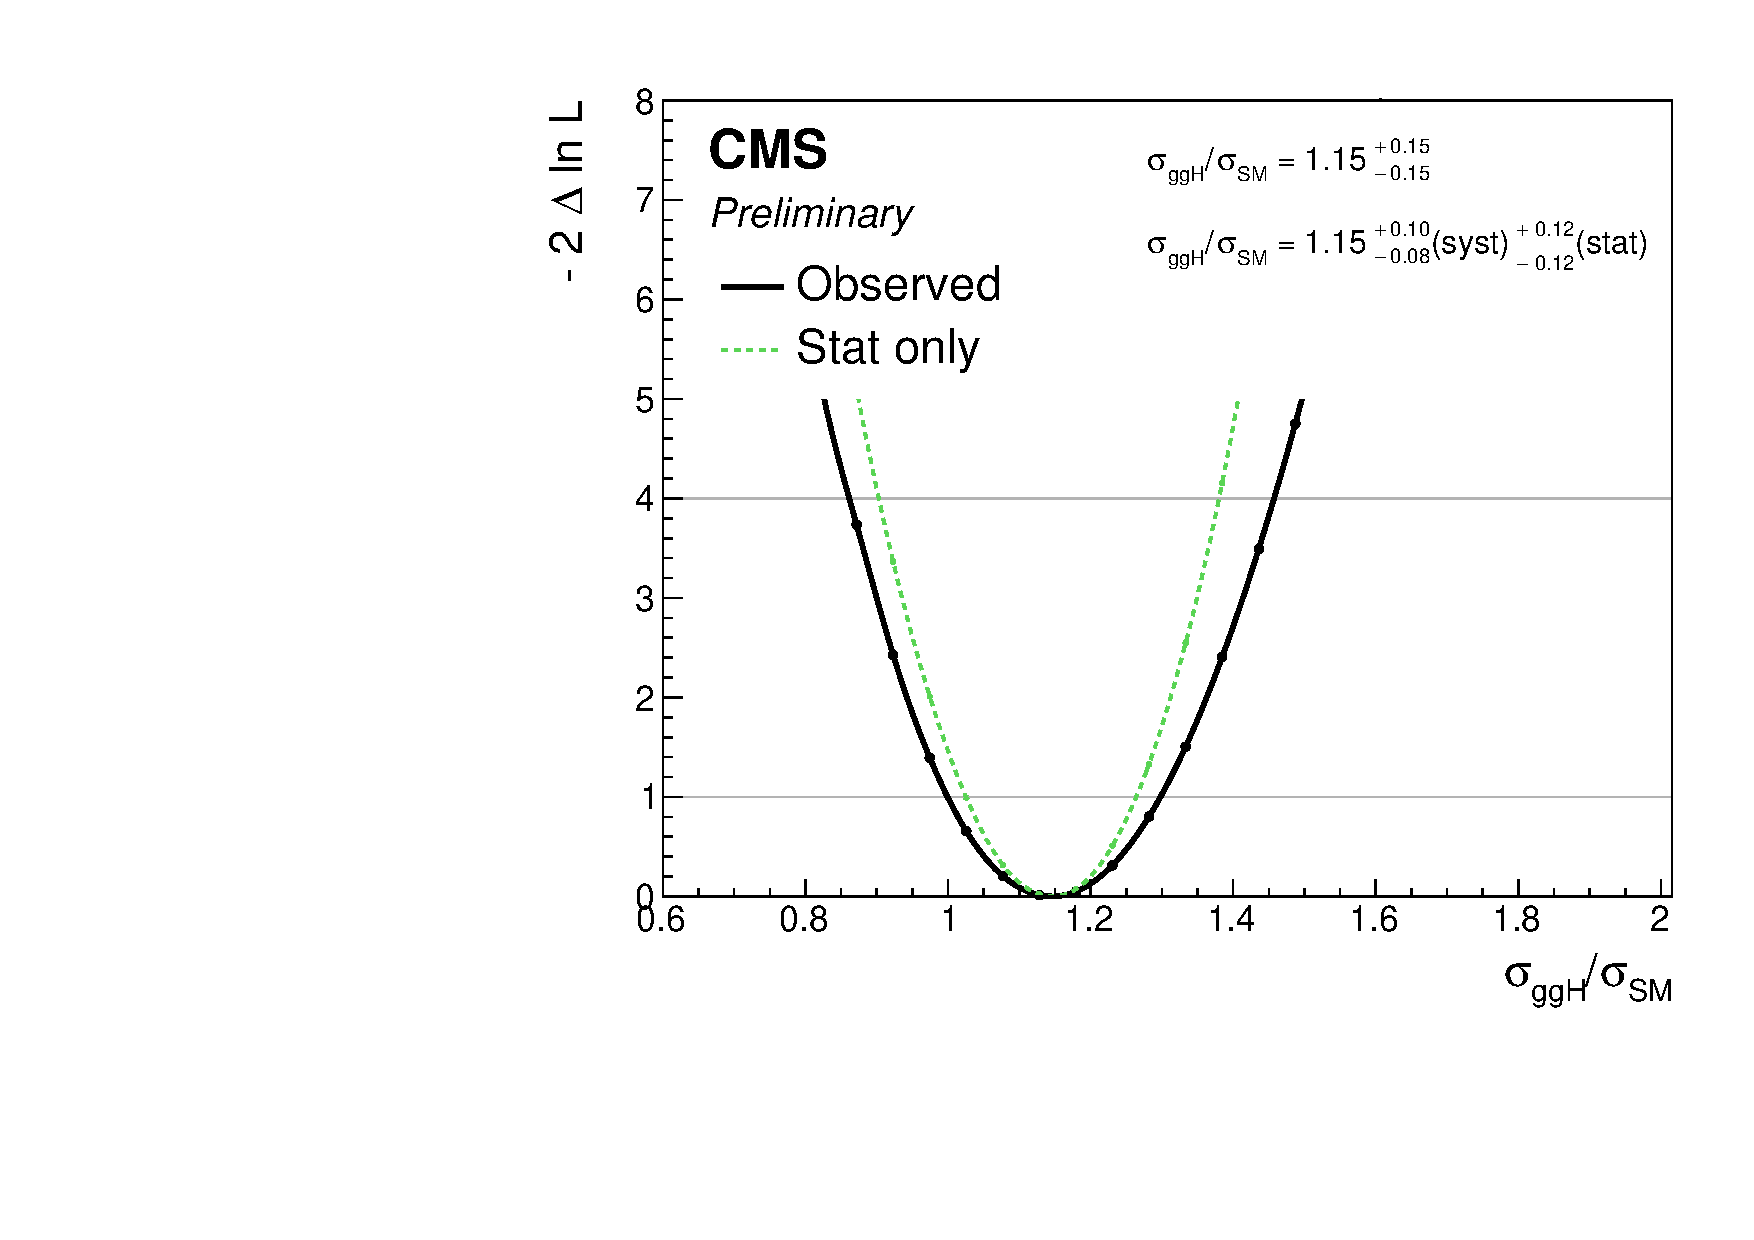
\includegraphics[width=\textwidth]{Figures/Results/ObsStage0_r_ggH.pdf}
  \caption[Likelihood scan for the ggH parameter in a two-parameter fit.]
  {
    The results of a two-parameter fit in the STXS framework,
    showing the scan of the profiled likelihood ratio in the ggH cross section.
    All ggH are grouped together in the fit to form one parameter, 
    with VBF bins comprising the second parameter.
    The ggH parameter includes bbH components, 
    while the qqH parameter includes the hadronic VH contribution. 
    The ttH, tH and VH leptonic processes are constrained to the SM prediction. 
    The solid black line shows the full scan, 
    whilst the dashed green line shows the scan without any systematic uncertainties included.
  }
  \label{fig:results_Stage0_ggH}
\end{figure}

\begin{figure}[hptb]
  \centering
  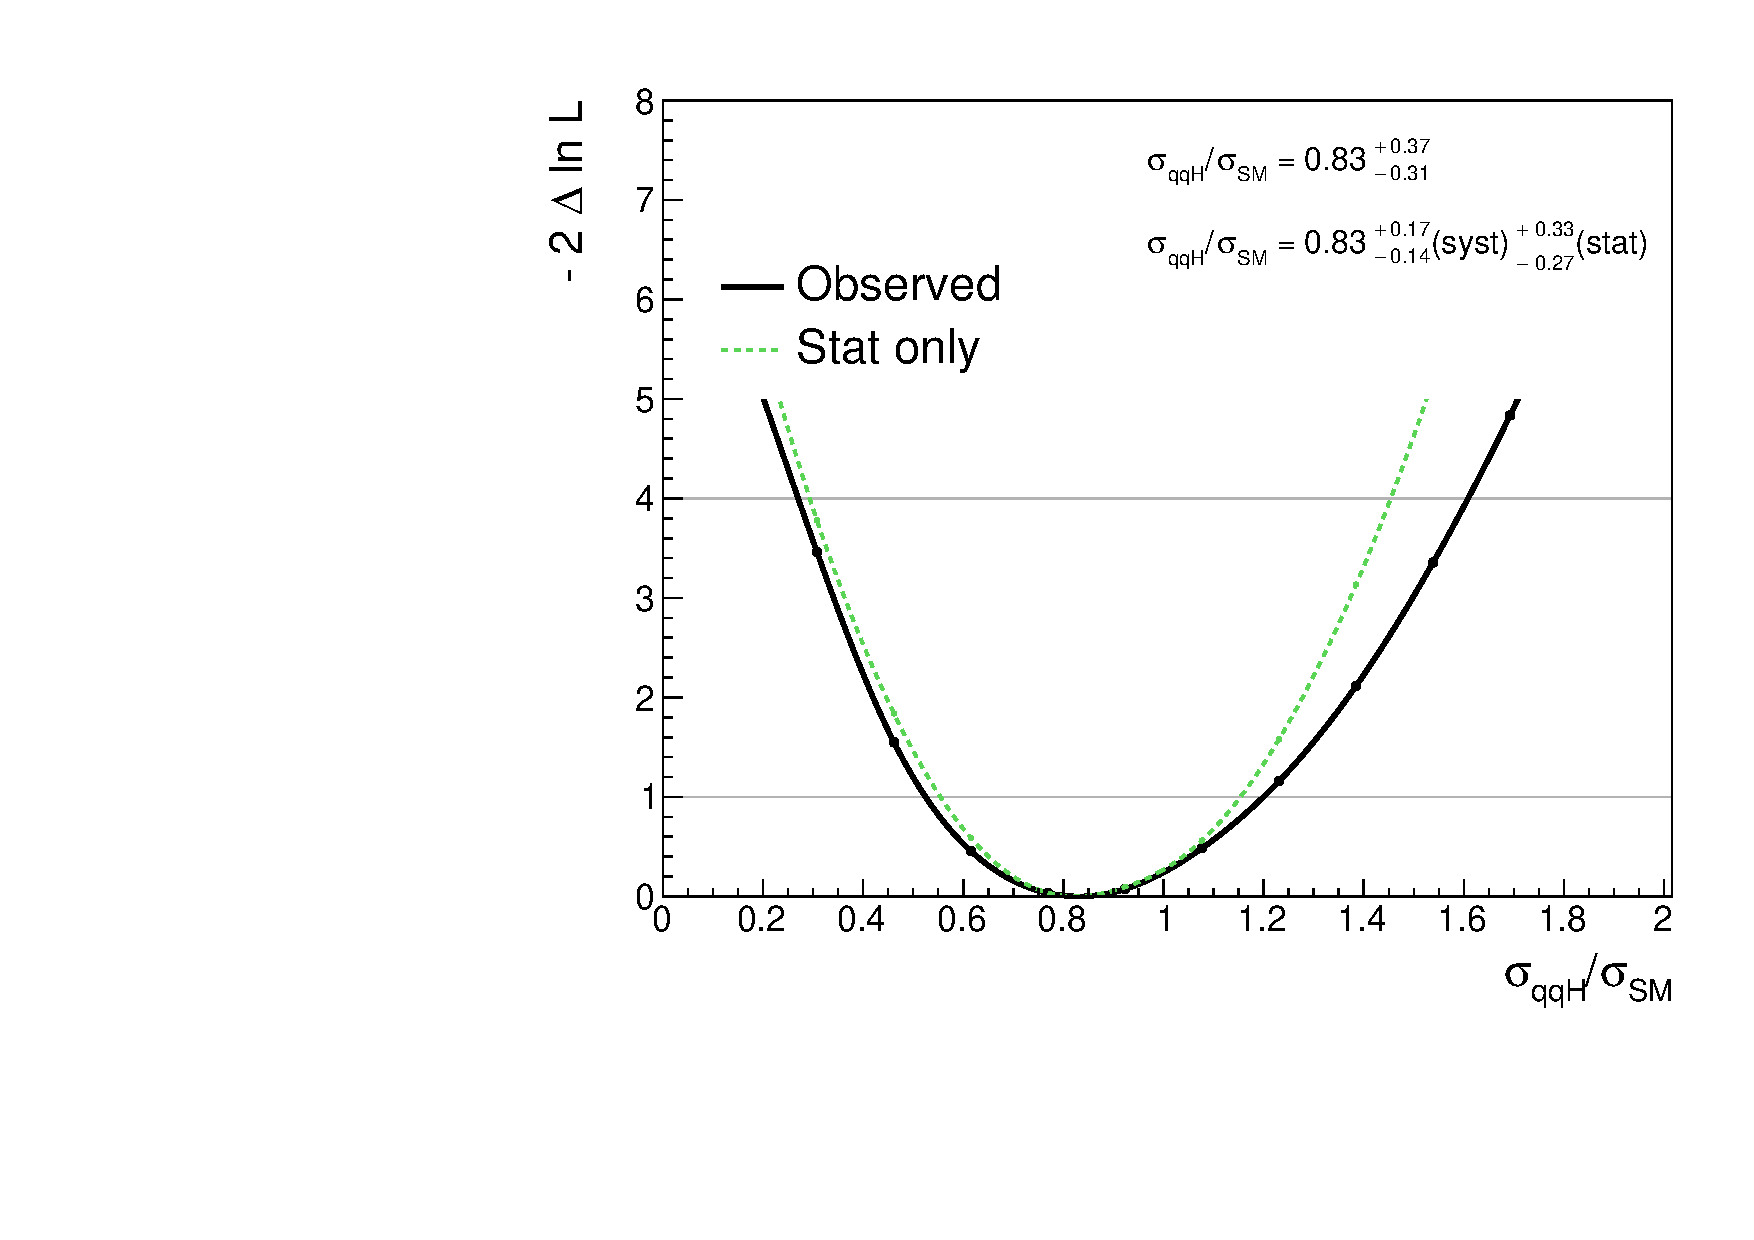
\includegraphics[width=\textwidth]{Figures/Results/ObsStage0_r_qqH.pdf}
  \caption[Likelihood scan for the qqH parameter in a two-parameter fit.]
  {
    The results of a two-parameter fit in the STXS framework,
    showing the scan of the profiled likelihood ratio in the qqH cross section.
    All ggH are grouped together in the fit to form one parameter, 
    with VBF bins comprising the second parameter.
    The ggH parameter includes bbH components, 
    while the qqH parameter includes the hadronic VH contribution. 
    The ttH, tH and VH leptonic processes are constrained to the SM prediction. 
    The solid black line shows the full scan, 
    whilst the dashed green line shows the scan without any systematic uncertainties included.
  }
  \label{fig:results_Stage0_qqH}
\end{figure}

\subsection{Stage 1 cross sections}

Two different measurements are performed at stage 1 of the STXS framework.
In both cases, some stage 1 bins are merged 
in order to improve the statistical sensitivity of the measurement.
In the first fit, the definition of parameters is motivated by merging as few bins as possible
whilst maintaining the uncertainty on each parameter at less than 100\% of the SM predicted value.
This results in a total of seven signal parameters.
There are six ggH parameters, of which four correspond to a single stage 1 bin;
these are the zero-jet (0J), one-jet low (1J low), medium (1J med), and high (1J high) \ptH bins.
The two-jet or greater parameter (GE2J) groups together five individual stage 1 bins, 
comprising the low, medium and high \ptH bins as well as the two VBF-like bins.
The ggH BSM parameter is the sum of the one-jet and two-jet ``beyond standard model" bins
where $\ptH > \SI{200}{GeV}$.
Finally, the qqH parameter is unchanged from stage 0;
all five bins are grouped together.
The results of this seven-parameter fit are shown in Figure~\ref{fig:results_stage1}. 
The observed 68\% CL intervals for each parameter are compared 
to the SM predictions and their associated uncertainties.
There is very good agreement with the SM; 
the $p$-value with respect to the SM hypothesis is approximately 64\%. %TODO revise how this is done
Furthermore, for several parameters, the experimental precision is less than a factor of three 
greater than the theoretical uncertainty on the SM prediction. %CONSEQUENCES

\begin{figure}[hptb]
  \centering
  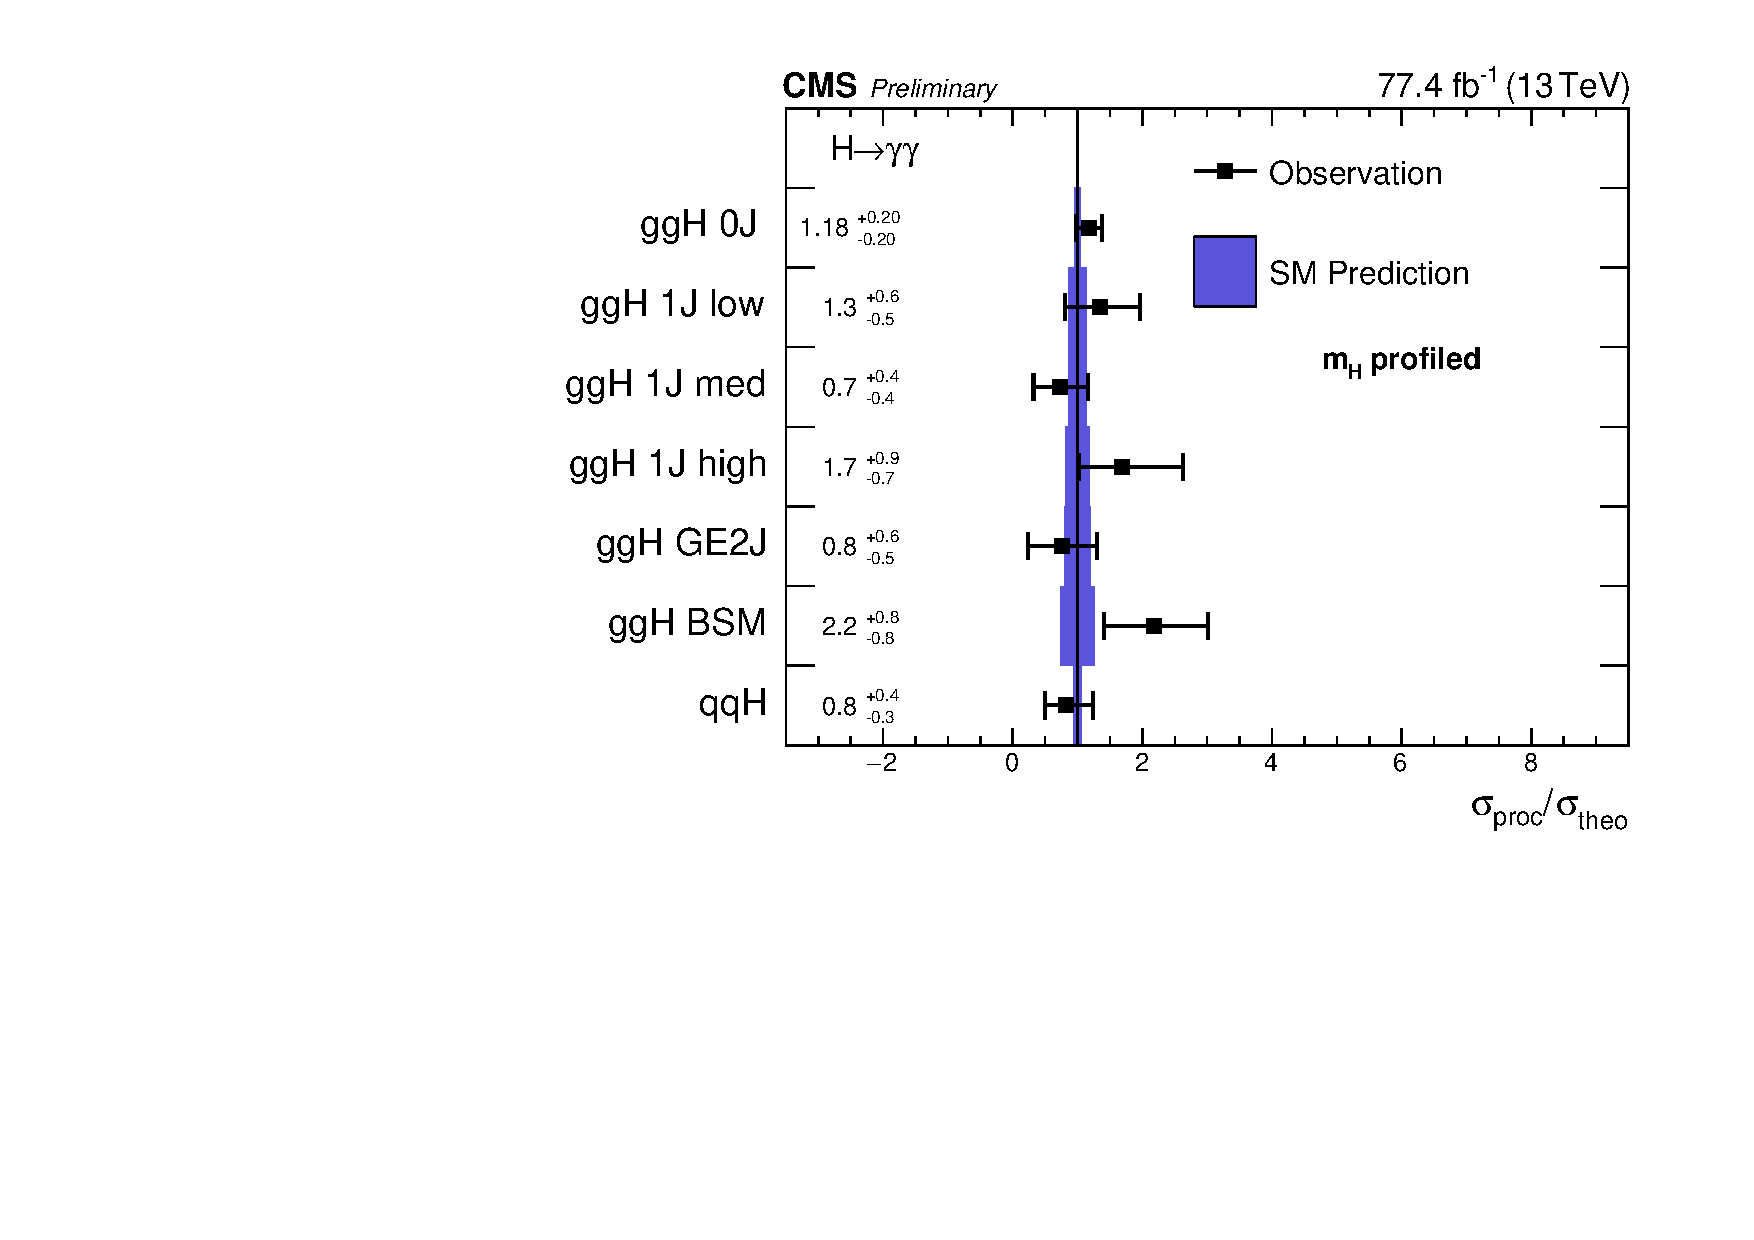
\includegraphics[width=\textwidth]{Figures/Results/Stage1.pdf}
  \caption[Results of a seven-parameter fit in the STXS framework.]
  {
    The results of a seven-parameter fit in the STXS framework. 
    The ggH 1J and 2J BSM bins are grouped together in the fit; 
    the remaining five ggH bins with two or more jets are also grouped. 
    All five VBF bins are grouped together. 
    The ggH parameters include bbH components, 
    while the qqH parameter includes the hadronic VH contribution. 
    The ttH, tH and VH leptonic processes are constrained to the SM prediction. 
    Cross section ratios are shown with approximate 68\% CL intervals (black points), 
    and compared to the SM expectations and their uncertainties (blue bands).
    The compatibility of this fit with the SM prediction, 
    expressed as a $p$-value with respect to the SM, is approximately 64\%.
    Figure first shown in Ref.~\cite{HIG-18-029}.
  }
  \label{fig:results_stage1}
\end{figure}

In the second measurement at stage 1, the fit contains thirteen signal parameters.
This choice represents the minimal possible merging of bins 
whilst retaining a reasonable sensitivity of less than around 200\% of the SM prediction.
Nine of the parameters correspond to individual ggH stage 1 bins; 
the only merged ggH parameter is the so-called ggH VBF-like parameter, 
where the 2J-like and 3J-like ggH VBF-like bins are grouped together.
For qqH, the 2J-like and 3J-like parameters represent individual bins, 
while the ``qqH other" parameter is composed of the VH-like, Rest and BSM bins.
The resulting cross sections normalised to the corresponding SM predictions 
are shown in Figure~\ref{fig:results_stage1min}.
In the fit all parameters are constrained to be non-negative -- this is necessary 
to ensure the fit converges.
The parameters whose best-fit values are constrained to be zero are known to have 68\% CL intervals 
which slightly under-cover. 
This is checked and confirmed using an ensemble of pseudo-experiments.
Therefore the compatibility of those parameters with the SM prediction is higher than 
the quoted 68\% CL intervals would imply.
The compatibility of the thirteen-parameter fit with the SM prediction, 
expressed as a $p$-value with respect to the SM hypothesis, is approximately 18\%.

%TODO switch this to one where VBF BSM is ungrouped?

\begin{figure}[hptb]
  \centering
  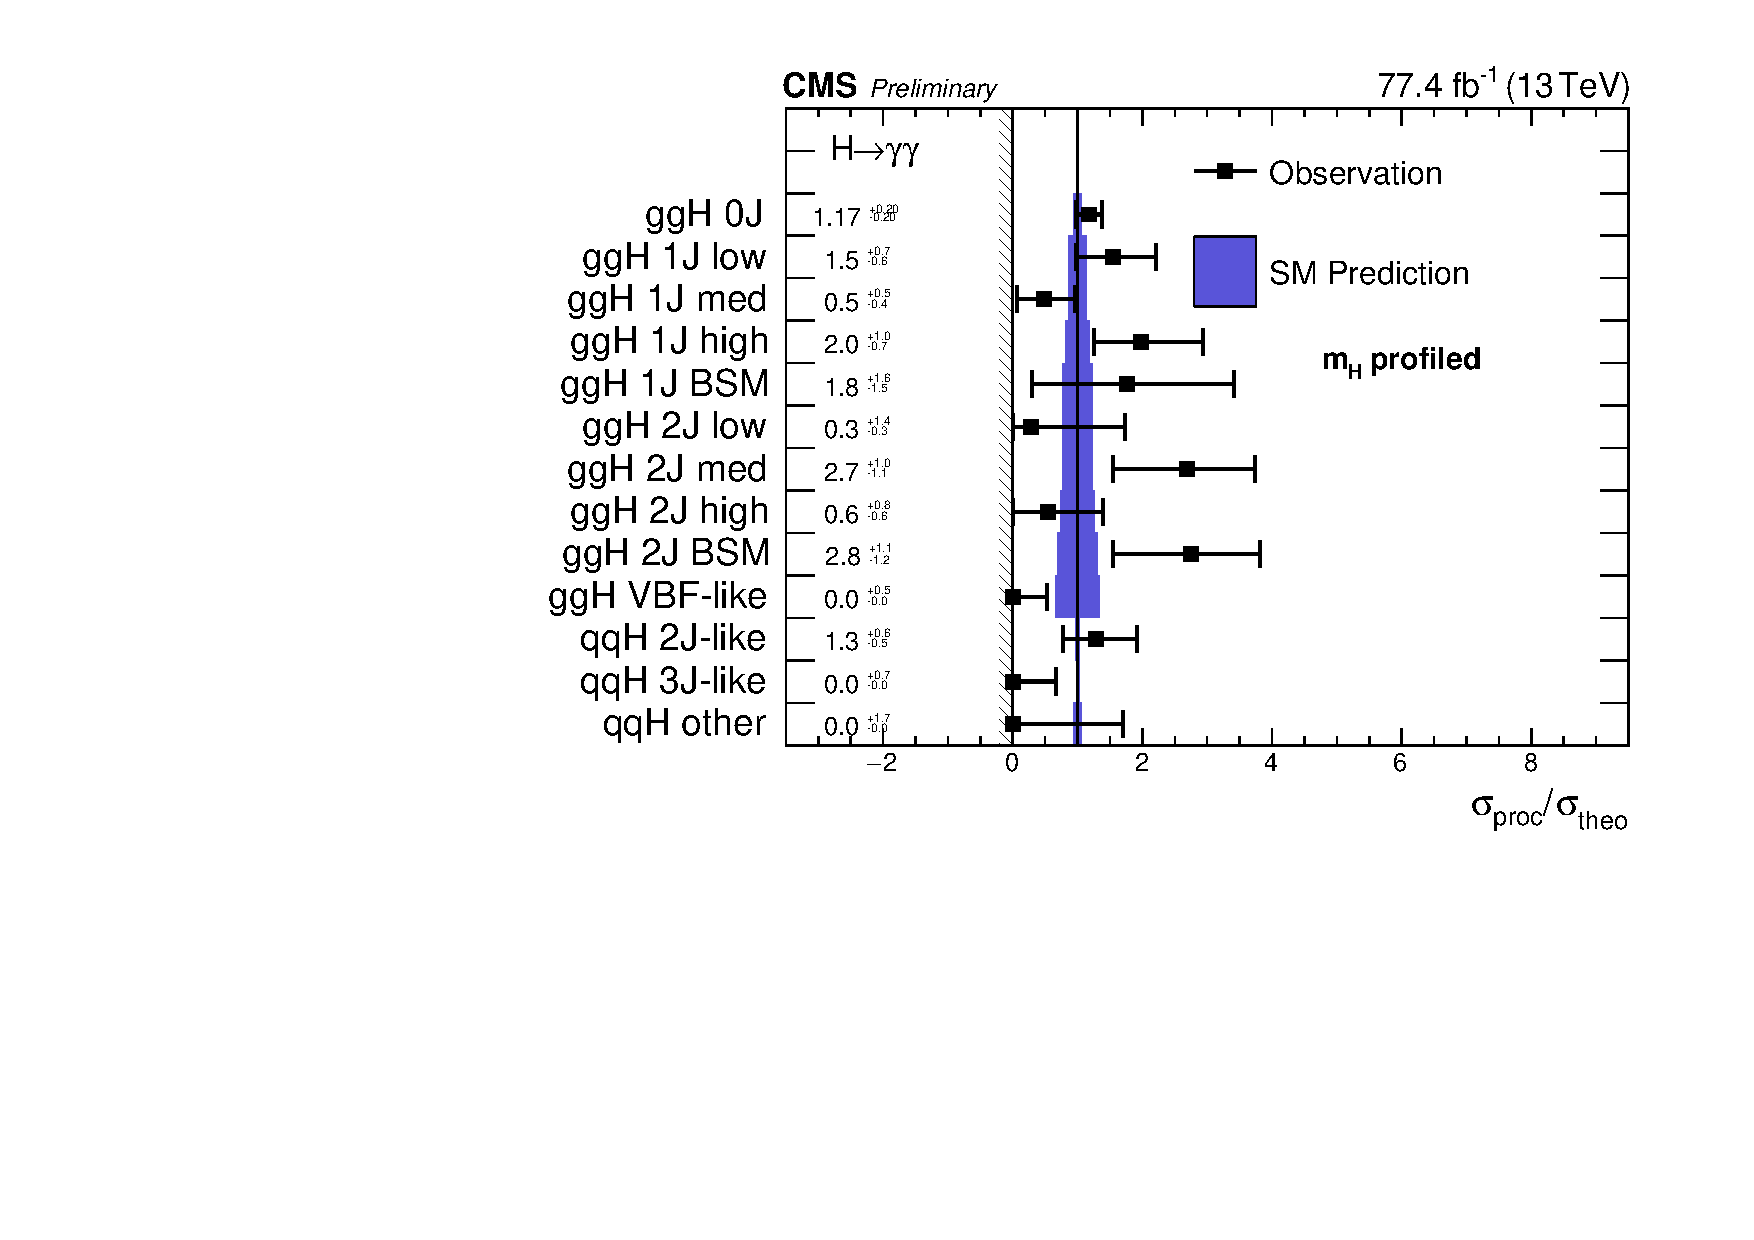
\includegraphics[width=\textwidth]{Figures/Results/Stage1Min.pdf}
  \caption[Results of a thirteen-parameter fit in the STXS framework.]
  {
    The results of a thirteen-parameter fit in the STXS framework. 
    The two VBF-like ggH bins are grouped to form one parameter, 
    as are the VBF BSM-like, VH-like and Rest bins.
    No further merging is performed. 
    The ggH parameters include bbH components, 
    while the qqH parameters include the hadronic VH contribution. 
    The ttH, tH and VH leptonic processes are constrained to the SM prediction. 
    Cross section ratios are shown with approximate 68\% CL intervals (black points) 
    and compared to the SM expectations and their uncertainties (blue bands). 
    The cross section ratios are constrained to be non-negative, 
    as indicated by the vertical line and hashed pattern. 
    The parameters whose best-fit values are at zero are known to have 68\% CL intervals 
    which slightly under-cover; this is checked using pseudo-experiments. 
    The compatibility of this fit with the SM prediction, 
    expressed as a $p$-value with respect to the SM, is approximately 18\%.
    Figure first shown in Ref.~\cite{HIG-18-029}.
  }
  \label{fig:results_stage1min}
\end{figure}

In addition to the best-fit values and 68\% CL intervals of each fit, 
the correlation between parameters is reported.
The correlation matrices are essential for reinterpretation of the measurements, 
where typically a rescaling of the signal parameters is performed 
according to the predictions of a beyond standard model theory.
The likelihood can then be approximated using a multivariate Gaussian distribution 
in terms of the new signal parameters, 
provided the correlation information between the original parameters is available.
The observed correlations between the signal parameters is therefore shown for the
seven-parameter and thirteen-parameter scenarios 
in Figures~\ref{fig:results_CorrStage1} and \ref{fig:results_CorrStage1Min} respectively.
In the seven-parameter fit, the magnitudes of the correlations are generally small.
The contamination from ggH 0J events in the 1J low categories results in a slightly higher 
anti-correlation, whilst the difficulty in distinguishing ggH 2J production from VBF 
is illustrated in the high anti-correlation between the ggH 2J and qqH parameters.
The thirteen-parameter fit displays higher correlation values, 
partly due to the low sensitivity to the qqH other parameter.

\begin{figure}[hptb]
  \centering
  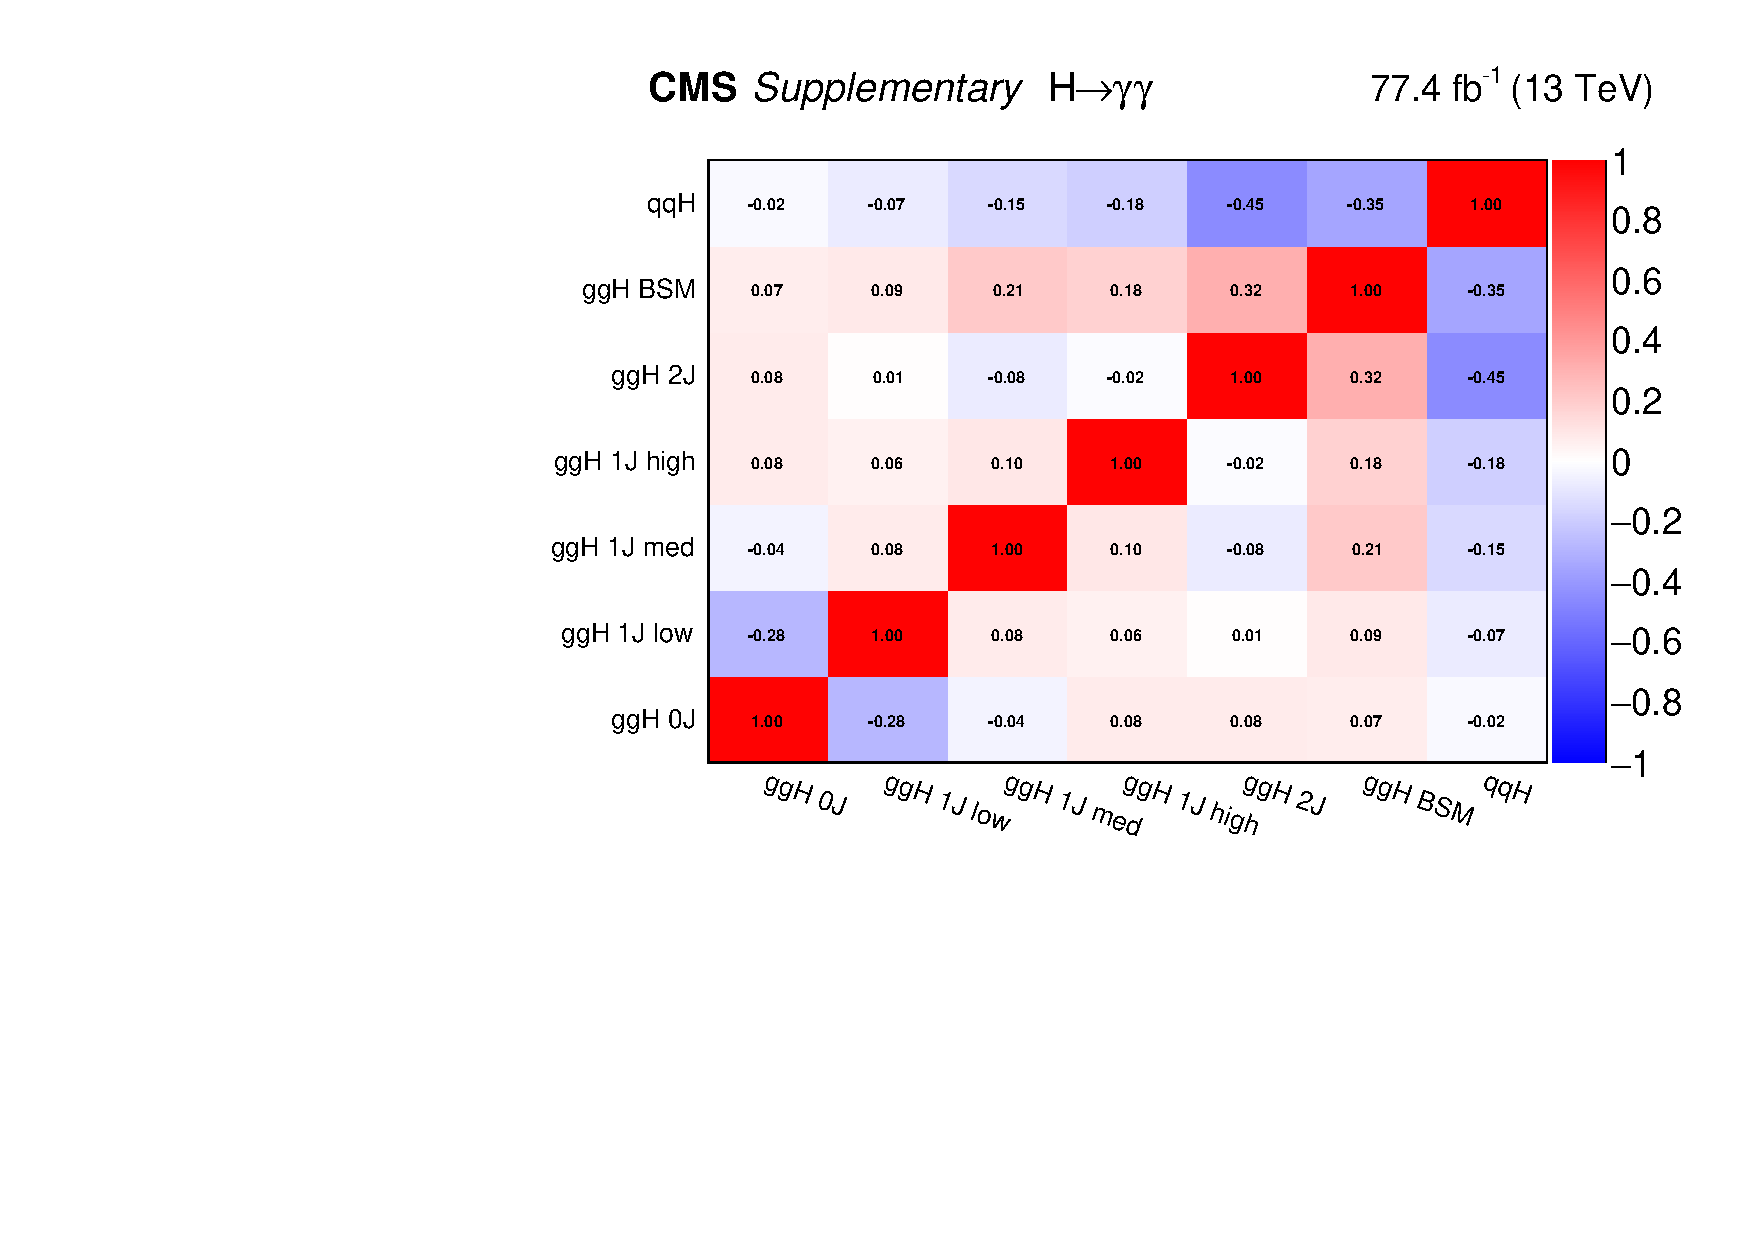
\includegraphics[width=\textwidth]{Figures/Results/CorrStage1.pdf}
  \caption[Observed correlations in a seven-parameter fit in the STXS framework.]
  {
    Observed correlations in a seven-parameter fit in the STXS framework. 
    The ggH 1J and 2J BSM bins are grouped together in the fit; 
    the remaining five ggH bins with two or more jets are also grouped. 
    All five VBF bins are grouped together. 
    The ggH parameters include bbH components, 
    while the qqH parameter includes the hadronic VH contribution. 
    The ttH, tH and VH leptonic processes are constrained to the SM prediction. 
    The size of the correlation is indicated by the colour scale.
    Figure first shown in Ref.~\cite{HIG-18-029}.
  }
  \label{fig:results_CorrStage1}
\end{figure}

\begin{figure}[hptb]
  \centering
  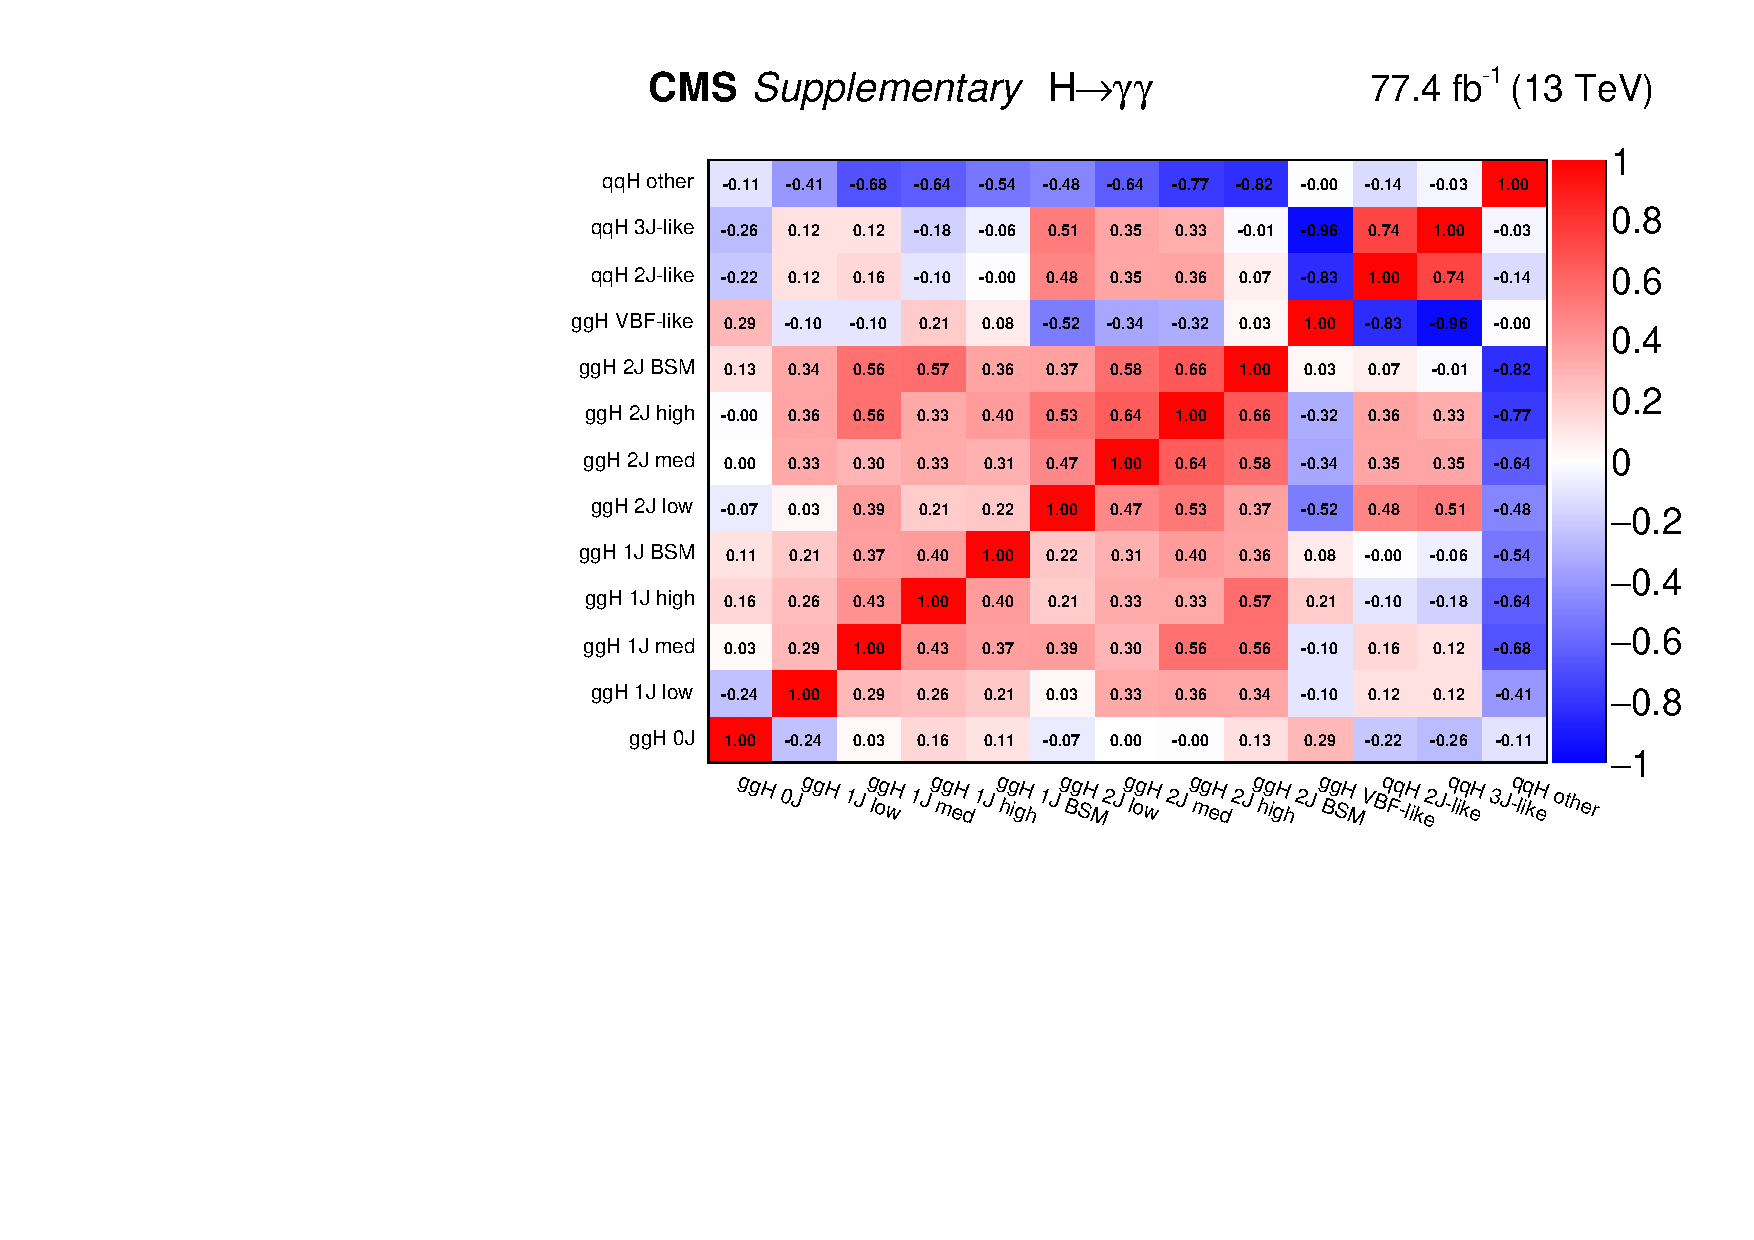
\includegraphics[width=\textwidth]{Figures/Results/CorrStage1Min.pdf}
  \caption[Observed correlations in a thirteen-parameter fit in the STXS framework.]
  {
    Observed correlations in a thirteen-parameter fit in the STXS framework. 
    The two VBF-like ggH bins are grouped to form one parameter, 
    as are the VBF BSM-like, VH-like and Rest bins. 
    No further merging is performed. 
    The ggH parameters include bbH components,
    while the qqH parameters include the hadronic VH contribution. 
    The ttH, tH and VH leptonic processes are constrained to the SM prediction. 
    The size of the correlation is indicated by the colour scale.
    Figure first shown in Ref.~\cite{HIG-18-029}.
  }
  \label{fig:results_CorrStage1Min}
\end{figure}

\section{Summary}

Measurements of cross sections at various levels of granularity within the STXS framework 
have been presented.
At stage 0, two parameters corresponding to ggH and electroweak qqH production are measured, 
with the observed values $\sigma_{ggH}/\sigma_{ggH}^{\textrm{SM}} = 1.15_{-0.15}^{+0.15}$ 
and $\sigma_{qqH}/\sigma_{qqH}^{\textrm{SM}} = 0.83_{-0.31}^{+0.37}$ 
highly consistent with the SM prediction.
At stage 1, two different fits with seven and thirteen signal parameters respectively are performed.
Both are consistent with the SM; the compatibility in terms of $p$-values with respect to the SM
hypothesis are 64\% and 18\% respectively.

The results at stage 1 of the STXS framework are summarised in Tables~\ref{tab:results_stage1}
and \ref{tab:results_stage1min}, 
where the measured cross section of each parameter is shown together with the SM prediction.
A breakdown of the uncertainties is also provided, with the total uncertainty split into 
its statistical, experimental, and theoretical components.

In this analysis, based upon the datasets collected by CMS in 2016 and 2017, 
no significant deviations from the SM predictions are observed.
The size of the uncertainties on stage 1 cross sections is still relatively large, 
and there is the scope for these to be substantially reduced in the near future.
This will be achieved by analysing the data collected during 2018, 
and then combining the results of multiple decay channels.
It is likely that the precision of some combined stage 1 cross section measurements will be 
comparable to the theoretical uncertainty on the SM prediction, 
which necessitates an effort to improve the theoretical predictions.
Furthermore, the statistical component of the uncertainties will decrease; 
in some cases, this will lead to systematic uncertainties limiting the measurement sensitivity.
Therefore an important aspect of future analyses will be in understanding 
and minimising the impact of these systematic uncertainties.
This will become crucial in the longer term, with Run 3 of the LHC due to commence in 2021, 
and the HL-LHC due to eventually provide an integrated luminosity of \SI{3000}{\fbinv} by 2040.
With these datasets, stringent tests of the SM at the level of a few per-cent 
are expected to be feasible~\cite{FutureYR}.

%TODO add the SM uncertainties to the tables

\begin{table}
\centering
  \begin{tabular}{ l | c | c | c | c | c | c | c }
\multirow{2}{*}{Signal parameter} & \multicolumn{2}{c}{Cross section (fb)}  & \multirow{2}{*}{$\sigma/\sigma_{\text{SM}}$}    & \multicolumn{4}{c}{Uncertainty on $\sigma/\sigma_{\text{SM}}$} \\
  & \multicolumn{1}{c}{SM pred.}  & \multicolumn{1}{c}{Measured} &          & \multicolumn{1}{c}{Total} & \multicolumn{1}{c}{Stat.} & \multicolumn{1}{c}{Exp.} & Theo.               \\
\hline
ggH 0J       & $61 \pm 3$                    & $72 \pm 12$                  & 1.18  & $_{-0.20}^{+0.20}$ & $_{-0.18}^{+0.18}$ & $_{-0.08}^{+0.10}$ & $_{-0.05}^{+0.06}$  \\[3pt]
ggH 1J low   & $15 \pm 2$                    & $21^{+9}_{-8}$               & 1.3   & $_{-0.5}^{+0.6}$   & $_{-0.5}^{+0.6}$   & $_{-0.2}^{+0.2}$   & $_{-0.1}^{+0.2}$    \\[3pt]
ggH 1J med   & $10 \pm 1$                    & $7.6^{+4.3}_{-4.1}$          & 0.7   & $_{-0.4}^{+0.4}$   & $_{-0.4}^{+0.4}$   & $_{-0.1}^{+0.1}$   & $_{-0.0}^{+0.1}$    \\[3pt]
ggH 1J high  & $1.7 \pm 0.3$                 & $2.9^{+1.6}_{-1.1}$          & 1.7   & $_{-0.7}^{+0.9}$   & $_{-0.6}^{+0.8}$   & $_{-0.2}^{+0.3}$   & $_{-0.1}^{+0.2}$    \\[3pt]
ggH 2J       & $11 \pm 2$                    & $8.4^{+6.1}_{-5.7}$          & 0.8   & $_{-0.5}^{+0.6}$   & $_{-0.5}^{+0.5}$   & $_{-0.1}^{+0.1}$   & $_{-0.1}^{+0.3}$    \\[3pt]
ggH BSM      & $1.3 \pm 0.4$                 & $2.9^{+1.1}_{-1.0}$          & 2.2   & $_{-0.8}^{+0.8}$   & $_{-0.6}^{+0.6}$   & $_{-0.3}^{+0.4}$   & $_{-0.2}^{+0.3}$    \\[3pt]
qqH          & $11 \pm 1$                    & $9.1^{+4.7}_{-3.0}$          & 0.8   & $_{-0.3}^{+0.4}$   & $_{-0.3}^{+0.4}$   & $_{-0.1}^{+0.2}$   & $_{-0.0}^{+0.1}$    \\[3pt]
\end{tabular}

  \caption[Results summary of a seven-parameter fit in the STXS framework.]
  {
    The results of a seven-parameter fit in the STXS framework. 
    The ggH 1J and 2J BSM bins are grouped together in the fit; 
    the remaining five ggH bins with two or more jets are also grouped. 
    All five VBF bins are grouped together. 
    The ggH parameters include bbH components, 
    while the qqH parameter includes the hadronic VH contribution. 
    The ttH, tH and VH leptonic processes are constrained to the SM prediction. 
    Both the measured value and the standard model prediction for 
    the product of the cross section and branching ratio are shown.
    The ratio of the measured cross section to the SM prediction is also shown, 
    together with its uncertainty.
    In addition, the statistical, experimental, and theoretical components 
    of the uncertainty on each parameter are reported.
    Table first shown in Ref.~\cite{HIG-18-029}.
  }
  \label{tab:results_stage1}
\end{table}

\begin{table}
\centering
  \begin{tabular}{ l | c | c | c | c | c | c | c }
\multirow{2}{*}{Signal parameter} & \multicolumn{2}{c}{Cross section (fb)}  & \multirow{2}{*}{$\sigma/\sigma_{\text{SM}}$}    & \multicolumn{4}{c}{Uncertainty on $\sigma/\sigma_{\text{SM}}$} \\
             & \multicolumn{1}{c}{SM pred.}  & \multicolumn{1}{c}{Measured} &       & Total              & Stat.              & Exp.               & Theo.               \\
\hline
ggH 0J       & 61                            & 72                           & 1.17  & $_{-0.20}^{+0.20}$ & $_{-0.18}^{+0.18}$ & $_{-0.07}^{+0.08}$ & $_{-0.04}^{+0.06}$  \\[3pt]
ggH 1J low   & 15                            & 24                           & 1.5   & $_{-0.6}^{+0.7}$   & $_{-0.5}^{+0.6}$   & $_{-0.1}^{+0.2}$   & $_{-0.1}^{+0.2}$    \\[3pt]
ggH 1J med   & 10                            & 5.1                          & 0.5   & $_{-0.4}^{+0.5}$   & $_{-0.4}^{+0.4}$   & $_{-0.1}^{+0.1}$   & $_{-0.0}^{+0.1}$    \\[3pt]
ggH 1J high  & 1.7                           & 3.4                          & 2.0   & $_{-0.7}^{+1.0}$   & $_{-0.7}^{+0.8}$   & $_{-0.1}^{+0.3}$   & $_{-0.2}^{+0.4}$    \\[3pt]
ggH 1J BSM   & 0.4                           & 0.6                          & 1.8   & $_{-1.5}^{+1.7}$   & $_{-1.4}^{+1.5}$   & $_{-0.2}^{+0.3}$   & $_{-0.1}^{+0.4}$    \\[3pt]
ggH 2J low   & 2.9                           & 0.8                          & 0.3   & $_{-0.3}^{+1.5}$   & $_{-0.3}^{+1.4}$   & $_{-0.1}^{+0.3}$   & $_{-0.0}^{+0.3}$    \\[3pt]
ggH 2J med   & 4.6                           & 12                           & 2.6   & $_{-1.1}^{+1.1}$   & $_{-1.0}^{+1.0}$   & $_{-0.2}^{+0.3}$   & $_{-0.3}^{+0.4}$    \\[3pt]
ggH 2J high  & 2.3                           & 1.3                          & 0.6   & $_{-0.6}^{+0.8}$   & $_{-0.6}^{+0.7}$   & $_{-0.1}^{+0.2}$   & $_{-0.0}^{+0.3}$    \\[3pt]
ggH 2J BSM   & 1.0                           & 2.7                          & 2.8   & $_{-1.2}^{+1.1}$   & $_{-1.0}^{+0.8}$   & $_{-0.3}^{+0.3}$   & $_{-0.4}^{+0.5}$    \\[3pt]
ggH VBF-like & 1.5                           & 0                            & 0.0   & $_{-0.0}^{+0.5}$   & $_{-0.0}^{+0.5}$   & $_{-0.0}^{+0.2}$   & $_{-0.0}^{+0.1}$    \\[3pt]
qqH 2J-like  & 2.1                           & 2.6                          & 1.3   & $_{-0.5}^{+0.6}$   & $_{-0.4}^{+0.4}$   & $_{-0.3}^{+0.4}$   & $_{-0.1}^{+0.1}$    \\[3pt]
qqH 3J-like  & 0.8                           & 0                            & 0.0   & $_{-0.0}^{+0.7}$   & $_{-0.0}^{+0.6}$   & $_{-0.0}^{+0.2}$   & $_{-0.0}^{+0.0}$    \\[3pt]
qqH other    & 8.2                           & 0                            & 0.0   & $_{-0.0}^{+1.7}$   & $_{-0.0}^{+1.6}$   & $_{-0.0}^{+0.6}$   & $_{-0.0}^{+0.2}$    \\[3pt]
\end{tabular}

  \caption[Results summary of a thirteen-parameter fit in the STXS framework.]
  {
    The results of a thirteen-parameter fit in the STXS framework. 
    The two VBF-like ggH bins are grouped to form one parameter, 
    as are the VBF BSM-like, VH-like and Rest bins.
    No further merging is performed. 
    The ggH parameters include bbH components, 
    while the qqH parameters include the hadronic VH contribution. 
    The ttH, tH and VH leptonic processes are constrained to the SM prediction. 
    Both the measured value and the standard model prediction for 
    the product of the cross section and branching ratio are shown.
    The ratio of the measured cross section to the SM prediction is also shown, 
    together with its uncertainty.
    In addition, the statistical, experimental, and theoretical components 
    of the uncertainty on each parameter are reported.
    Table first shown in Ref.~\cite{HIG-18-029}.
  }
  \label{tab:results_stage1min}
\end{table}

%TODO put the mass distributions for each stage 1 fit scenario in an appendix?
